%----------------------------------------------------------------------------------------
%	PACKAGES AND THEMES
%----------------------------------------------------------------------------------------
\documentclass[aspectratio=128,xcolor=dvipsnames, notes]{beamer}
\usetheme{SimplePlus}
\usepackage{tikz} % for figures
\usepackage[style=authoryear, bibencoding=utf8, minnames=1, maxnames=3,
maxbibnames=99, natbib=true, dashed=false, terseinits=true,
firstinits=true, uniquename=false, uniquelist=true, labeldate=true,
doi=false, isbn=false, natbib=true, backend=biber, note=false, url=false, eprint=false]{biblatex}
\AtEveryBibitem{\clearlist{language}}
\AtEveryBibitem{%
  \clearfield{note}%
}
\usepackage{dsfont} % for fancy R
\addbibresource{references.bib} 
\usepackage{hyperref}
\usepackage{ragged2e}
\usepackage{enumerate}% http://ctan.org/pkg/enumerate
\usepackage{xcolor}
\usepackage{graphicx} % Allows including images
\usepackage{booktabs} % Allows the use of \toprule, \midrule and \bottomrule in tables

\setbeamertemplate{footline}[frame number]{}
\renewcommand*{\bibfont}{\scriptsize}
\newcommand{\highlight}[1]{%
  \colorbox{yellow!50}{$\displaystyle#1$}}
  \newcommand{\fundmat}{\mathbf{\Phi}(t, 0)}
\newcommand{\fundmats}{\mathbf{\Phi}(t, s)}
\newcommand{\fundmatso}{\mathbf{\Phi}(s, 0)}
\newcommand{\fundmatsu}{\mathbf{\Phi}(s, u)}
\newcommand{\fundmattv}{\mathbf{\Phi}(t, v)}
\newcommand{\Expec}{\mathbb{E}}
\newcommand{\Cov}{\operatorname{Cov}}

% New commands
\newcommand{\pkg}[1]{{\normalfont\fontseries{b}\selectfont #1}} \let\proglang=\textsf \let\code=\texttt
\newcommand{\1}{\mathbf{1}}
\newcommand{\boldbeta}{\boldsymbol{\beta}}
\newcommand{\boldut}{\mathbf{u}_i(t)}
\newcommand{\boldepst}{\boldsymbol{\varepsilon}_{ij}(t)}
\newcommand{\Expec}{\mathbb{E}}

\newcommand{\boldpsi}{\boldsymbol{\psi}}
\newcommand{\boldy}{\mathbf{y}}

\newcommand{\Var}{\operatorname{Var}}
\newcommand{\Cov}{\operatorname{Cov}}
\newcommand{\diag}{\operatorname{diag}}
\newcommand{\ICC}{\operatorname{ICC}}
\DeclareMathOperator{\vect}{vec}
%----------------------------------------------------------------------------------------
%	TITLE PAGE
%----------------------------------------------------------------------------------------

\title[short title]{Functional Regression Models in Human Movement Biomechanics} % The short title appears at the bottom of every slide, the full title is only on the title page
\subtitle{Methodology and Applications}

\author[Edward Gunning] {Edward Gunning}

% \institute[NTU] % Your institution as it will appear on the bottom of every slide, may be shorthand to save space
% {
%     Department of Mathematics and Statistics \\
%     University of Limerick % Your institution for the title page
% }
\date{
    \vskip1em
    JHU Biostatistics Wearable and Implantable Technology Group \\
    \vskip1em
    September $13^${th} $2024$
} % Date, can be changed to a custom date


%----------------------------------------------------------------------------------------
%	PRESENTATION SLIDES
%----------------------------------------------------------------------------------------

\begin{document}

\begin{frame}
    % Print the title page as the first slide
    \titlepage
\end{frame}

\section{Introduction}

\begin{frame}{Background}
\textcite{winter_biomechanics_1979} defines \textbf{human movement biomechanics} as
    \begin{quote}
        ``\dots the inter-discipline that describes, analyses, and assesses human movement" 
    \end{quote}

\begin{itemize}
    \pause \item Data collected on displacement, velocity and acceleration (\textbf{kinematics}) and forces (\textbf{kinetics}).
    \pause \item Continuously measured throughout a movement $\rightarrow$ smooth time-varying curves, very suitable for FDA.
\end{itemize}
\vfill
\pause \begin{figure}
    \centering
    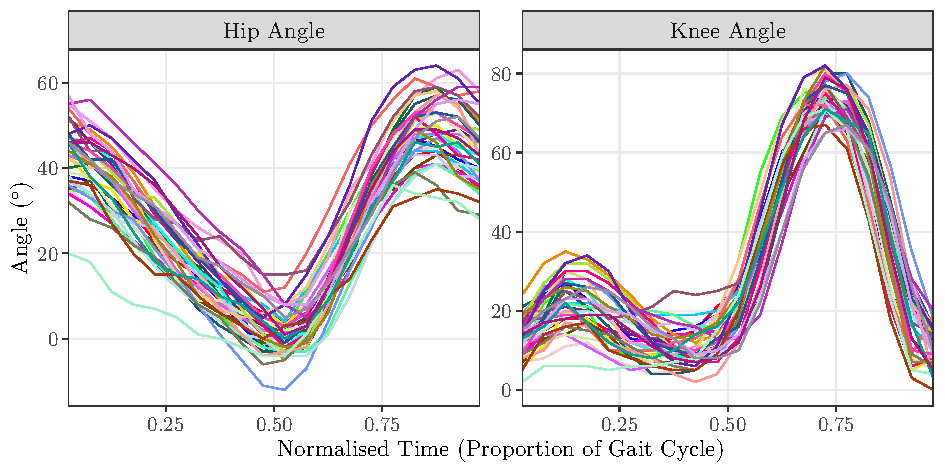
\includegraphics[width=0.5\textwidth, page = 1]{figures/thesis-chapt-1-2.pdf}
    \caption{The childrens' gait dataset \parencite{rice_estimating_1991}.}
    \label{fig:enter-label}
\end{figure}
\end{frame}



\begin{frame}[noframenumbering]{Background}
\textcite{winter_biomechanics_1979} defines \textbf{human movement biomechanics} as
    \begin{quote}
        ``\dots the inter-discipline that describes, analyses, and assesses human movement" 
    \end{quote}

\begin{itemize}
     \item Data collected on displacement, velocity and acceleration (\textbf{kinematics}) and forces (\textbf{kinetics}).
     \item Continuously measured throughout a movement $\rightarrow$ smooth time-varying curves, very suitable for FDA.
\end{itemize}
\vfill
 \begin{figure}
    \centering
    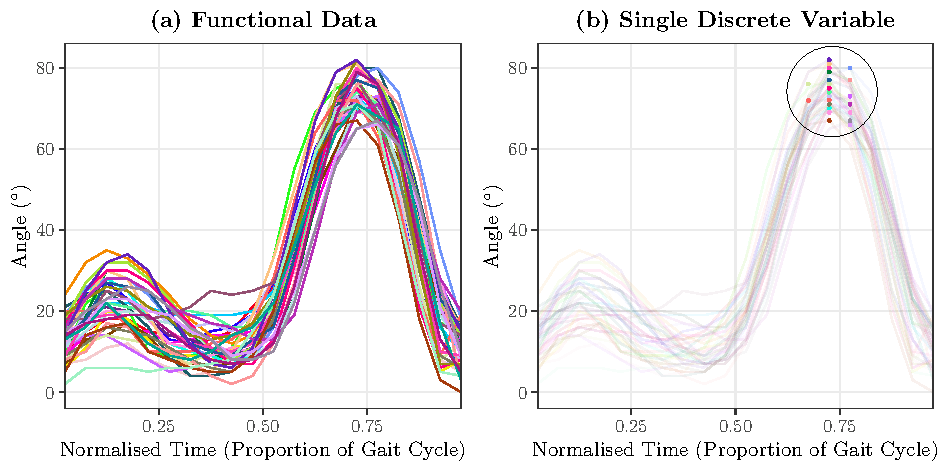
\includegraphics[width=0.5\textwidth]{figures/discrete-variable-plot.pdf}
    \caption{Data reduction of the knee angle curve to a single dicrete variable (peak knee flexion).}
    \label{fig:enter-label}
\end{figure}
\end{frame}

\begin{frame}{Second-Generation Functional Data in Biomechanics}
    \begin{columns}[c] % The "c" option specifies centered vertical alignment while the "t" option is used for top vertical alignment
        \centering
        \column{.33\textwidth} % Left column and width
        \centering
        \textbf{Volume} 
        \vskip1em
        \centering
        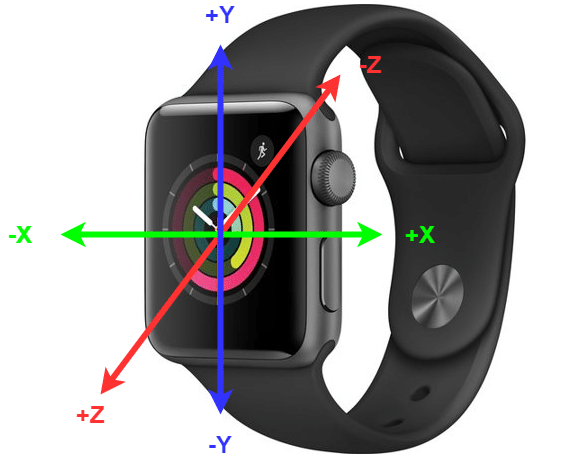
\includegraphics[width = 0.4 \textwidth]{figures/Apple-watch-series-1-used-for-recording-accelerometer-and-gyroscope-signals.png}
        \vskip1em
        \centering
        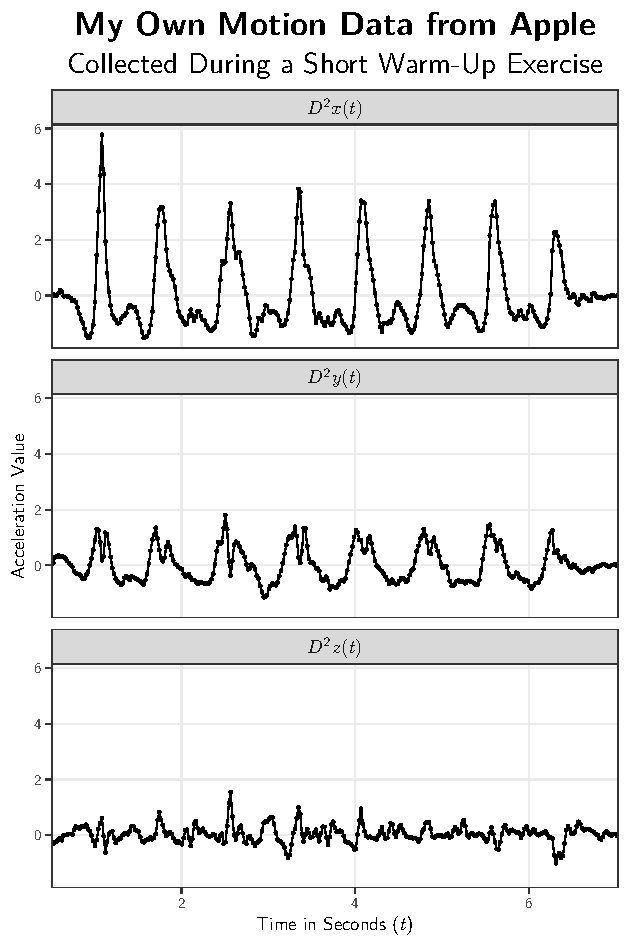
\includegraphics[width = 0.75\textwidth]{figures/my-apple-data.pdf}

        \pause \column{.33\textwidth} % Right column and width
        \centering
        \textbf{Complexity}
        \vskip1em
        \vfill
        \centering 
        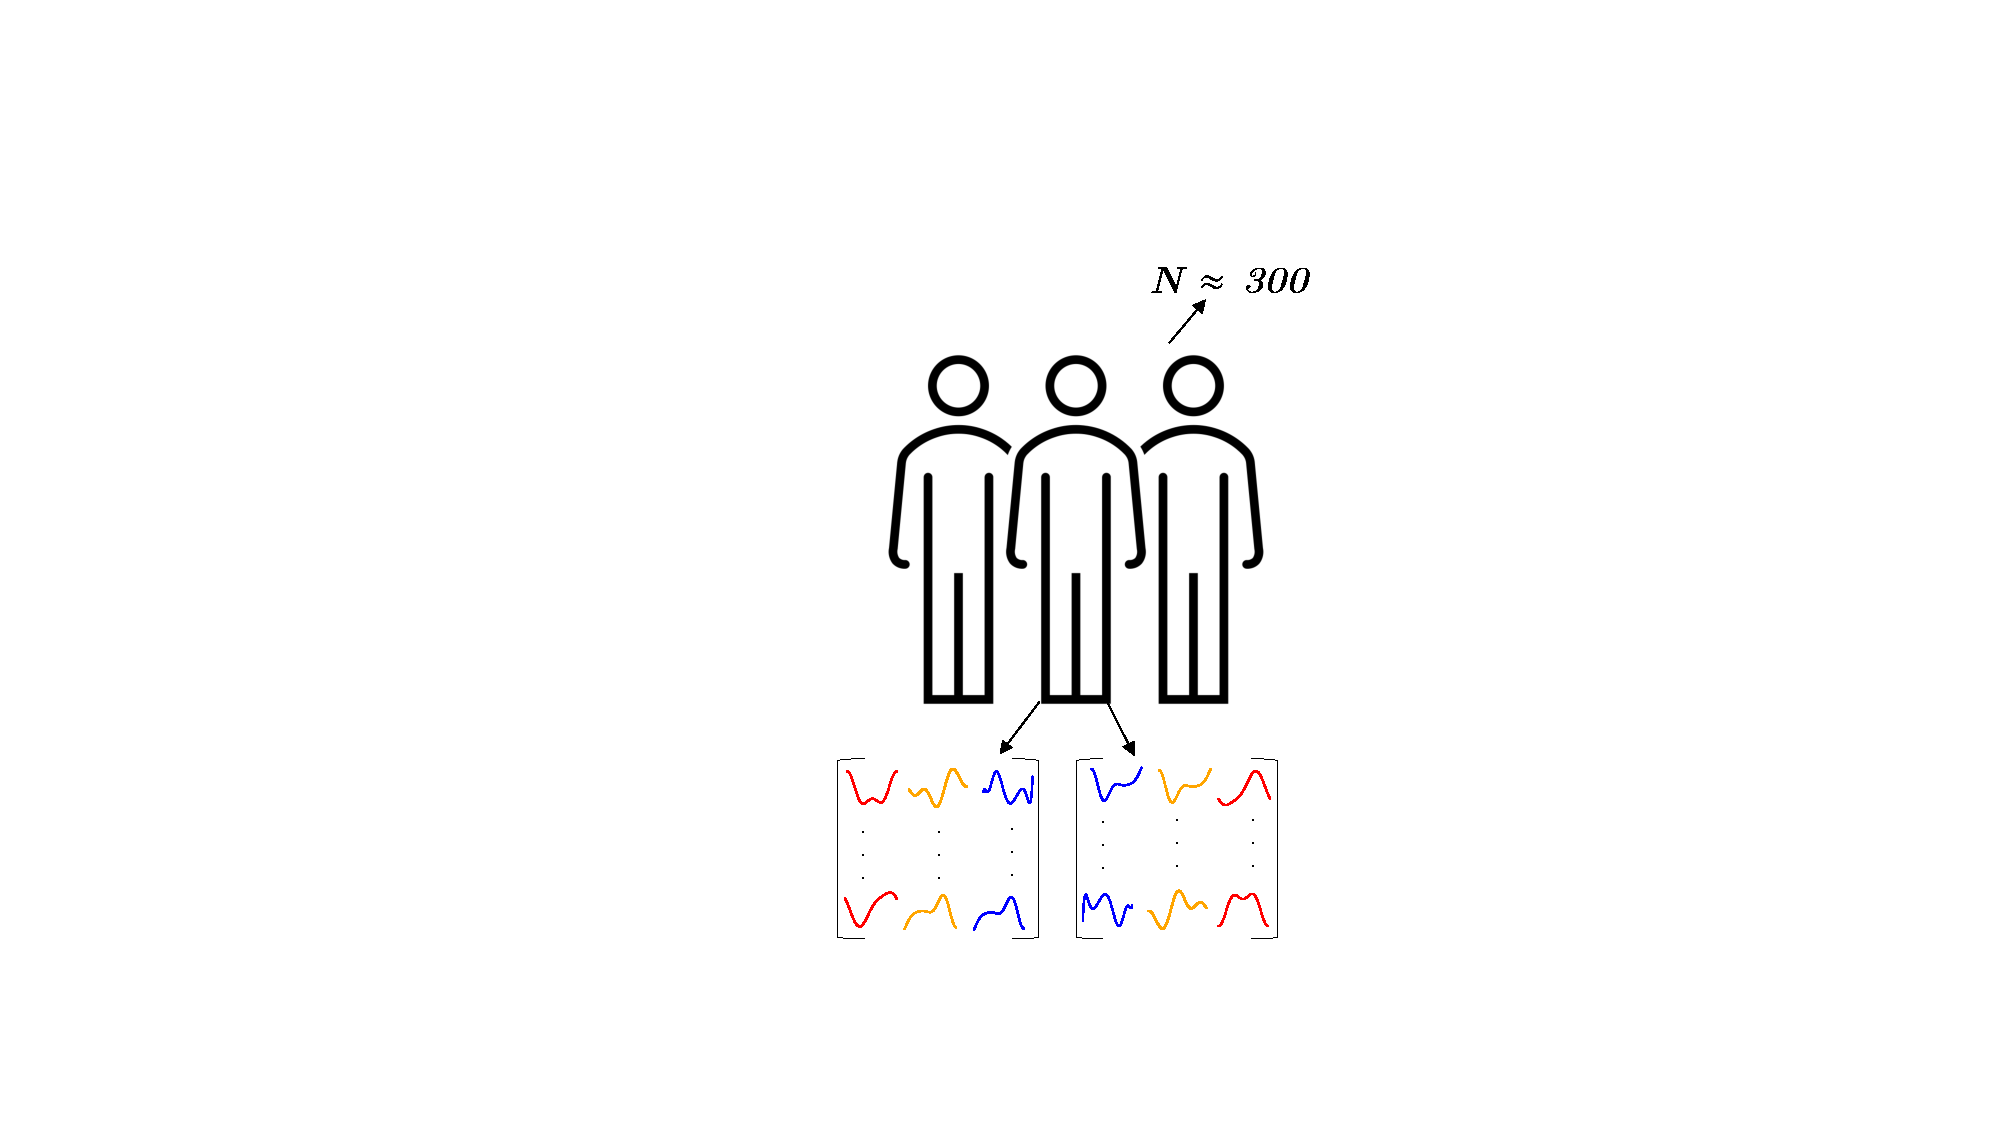
\includegraphics[width = 0.7\textwidth]{figures/Multilevel-Data-Figure.pdf}
        \vskip1em
        \centering
        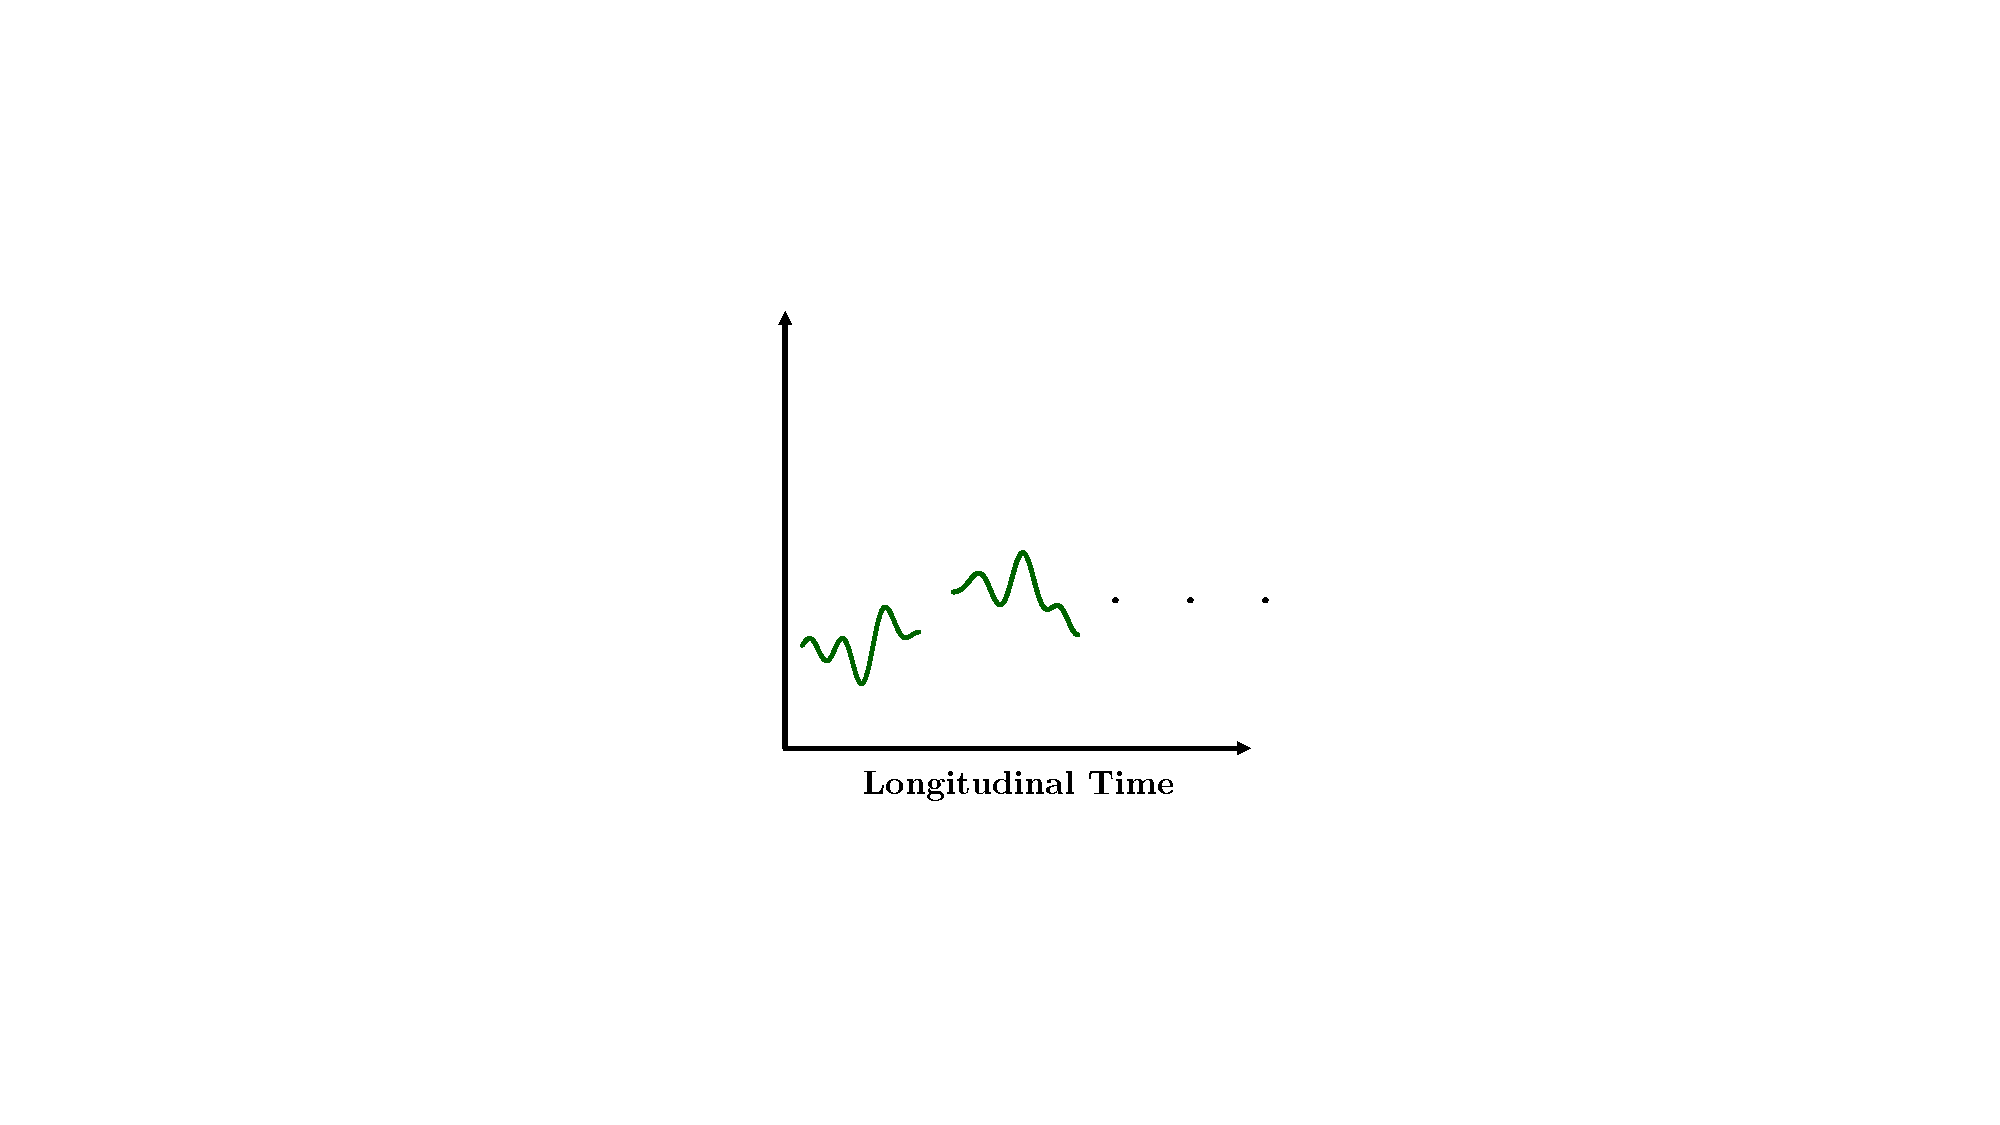
\includegraphics[width = 0.6\textwidth]{figures/Longitudinal-Figure.pdf}

        
        \pause \column{.33\textwidth} % Right column and width
        \centering
        \textbf{Variety}
        \vskip2em
        \centering
        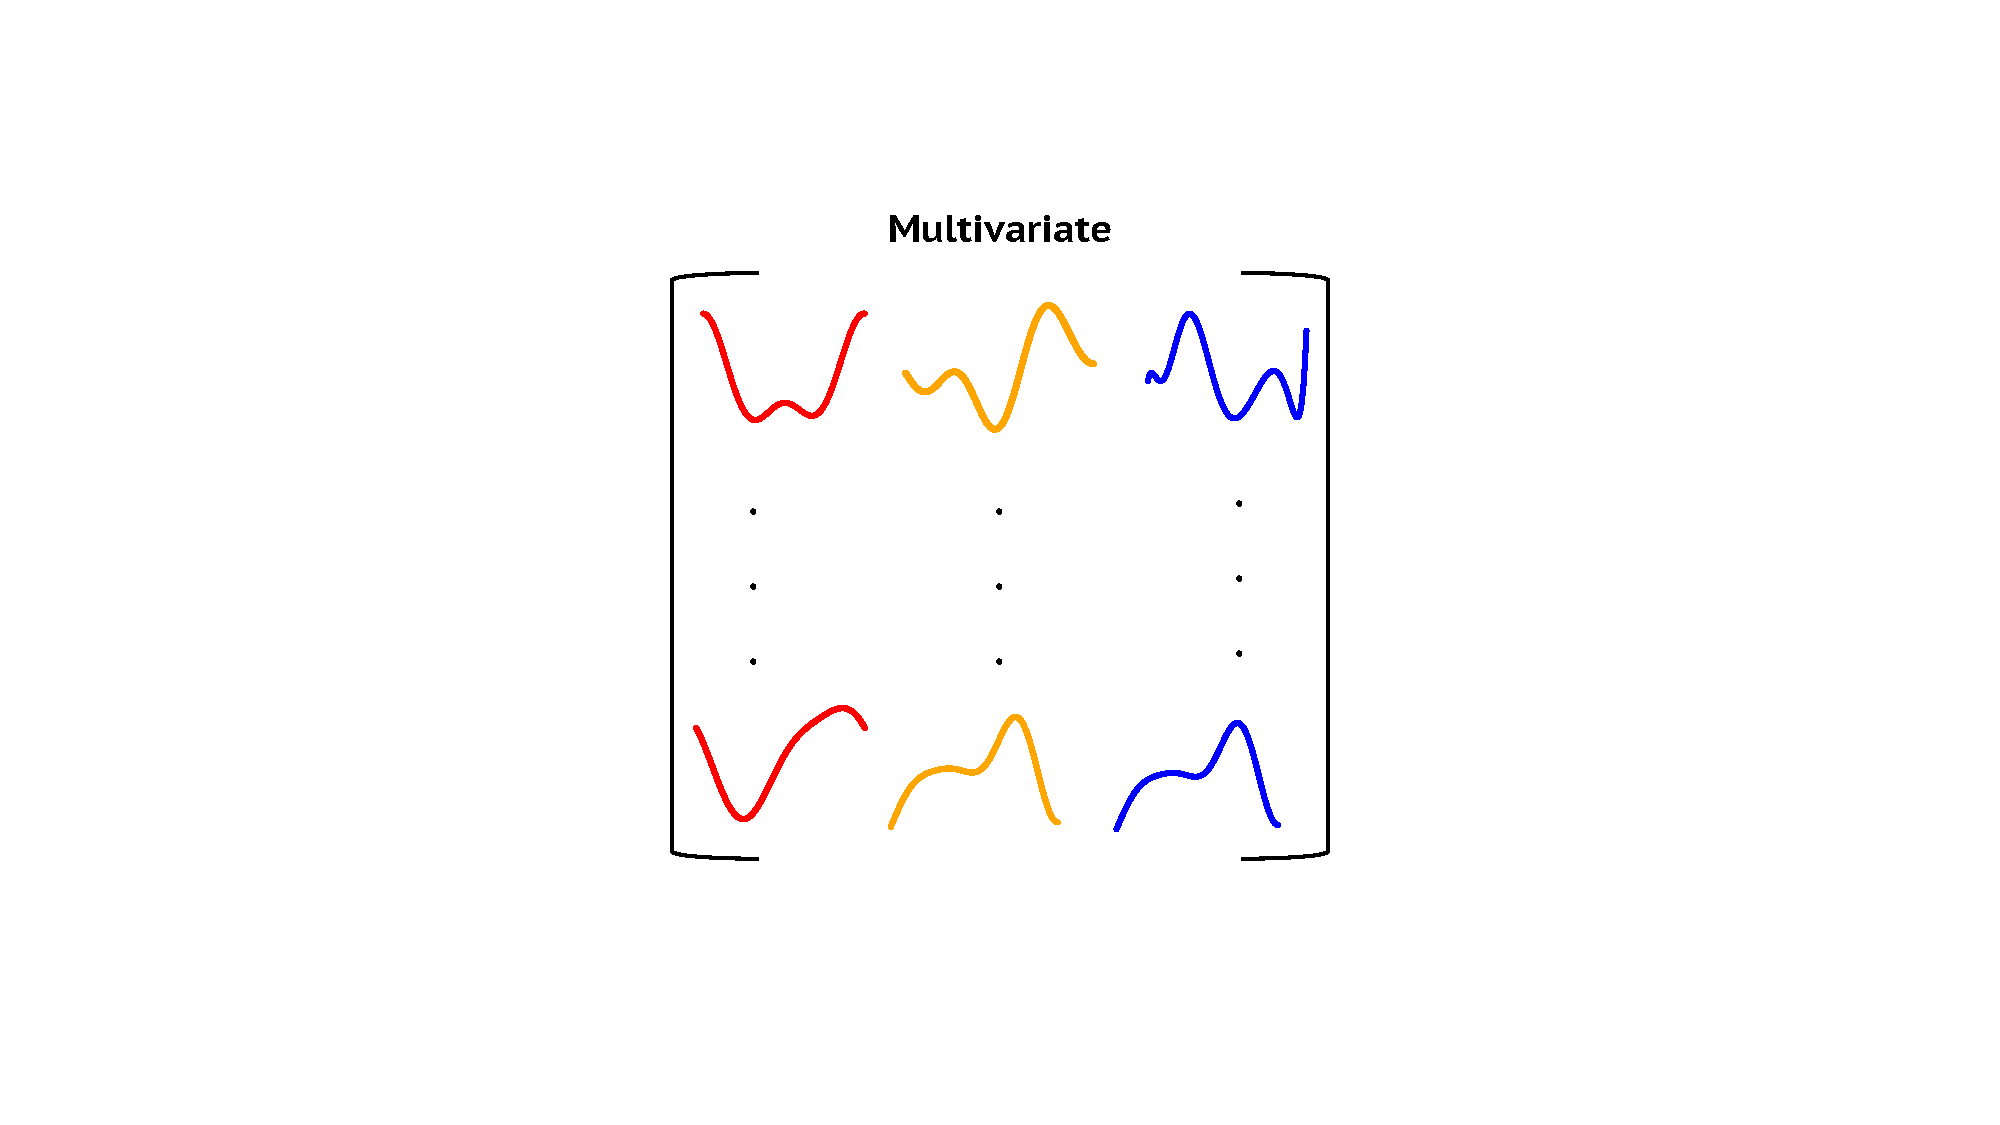
\includegraphics[width = 0.75\textwidth]{figures/Multivariate.pdf}
        \vskip1em
        Human movement as a system of multiple related parts $\rightarrow$ \textbf{multivariate} and \textbf{dynamical systems} approaches to analysis.
    \end{columns}
\end{frame}

\begin{frame}{Compare and Contrast}
    \begin{figure}
        \centering
        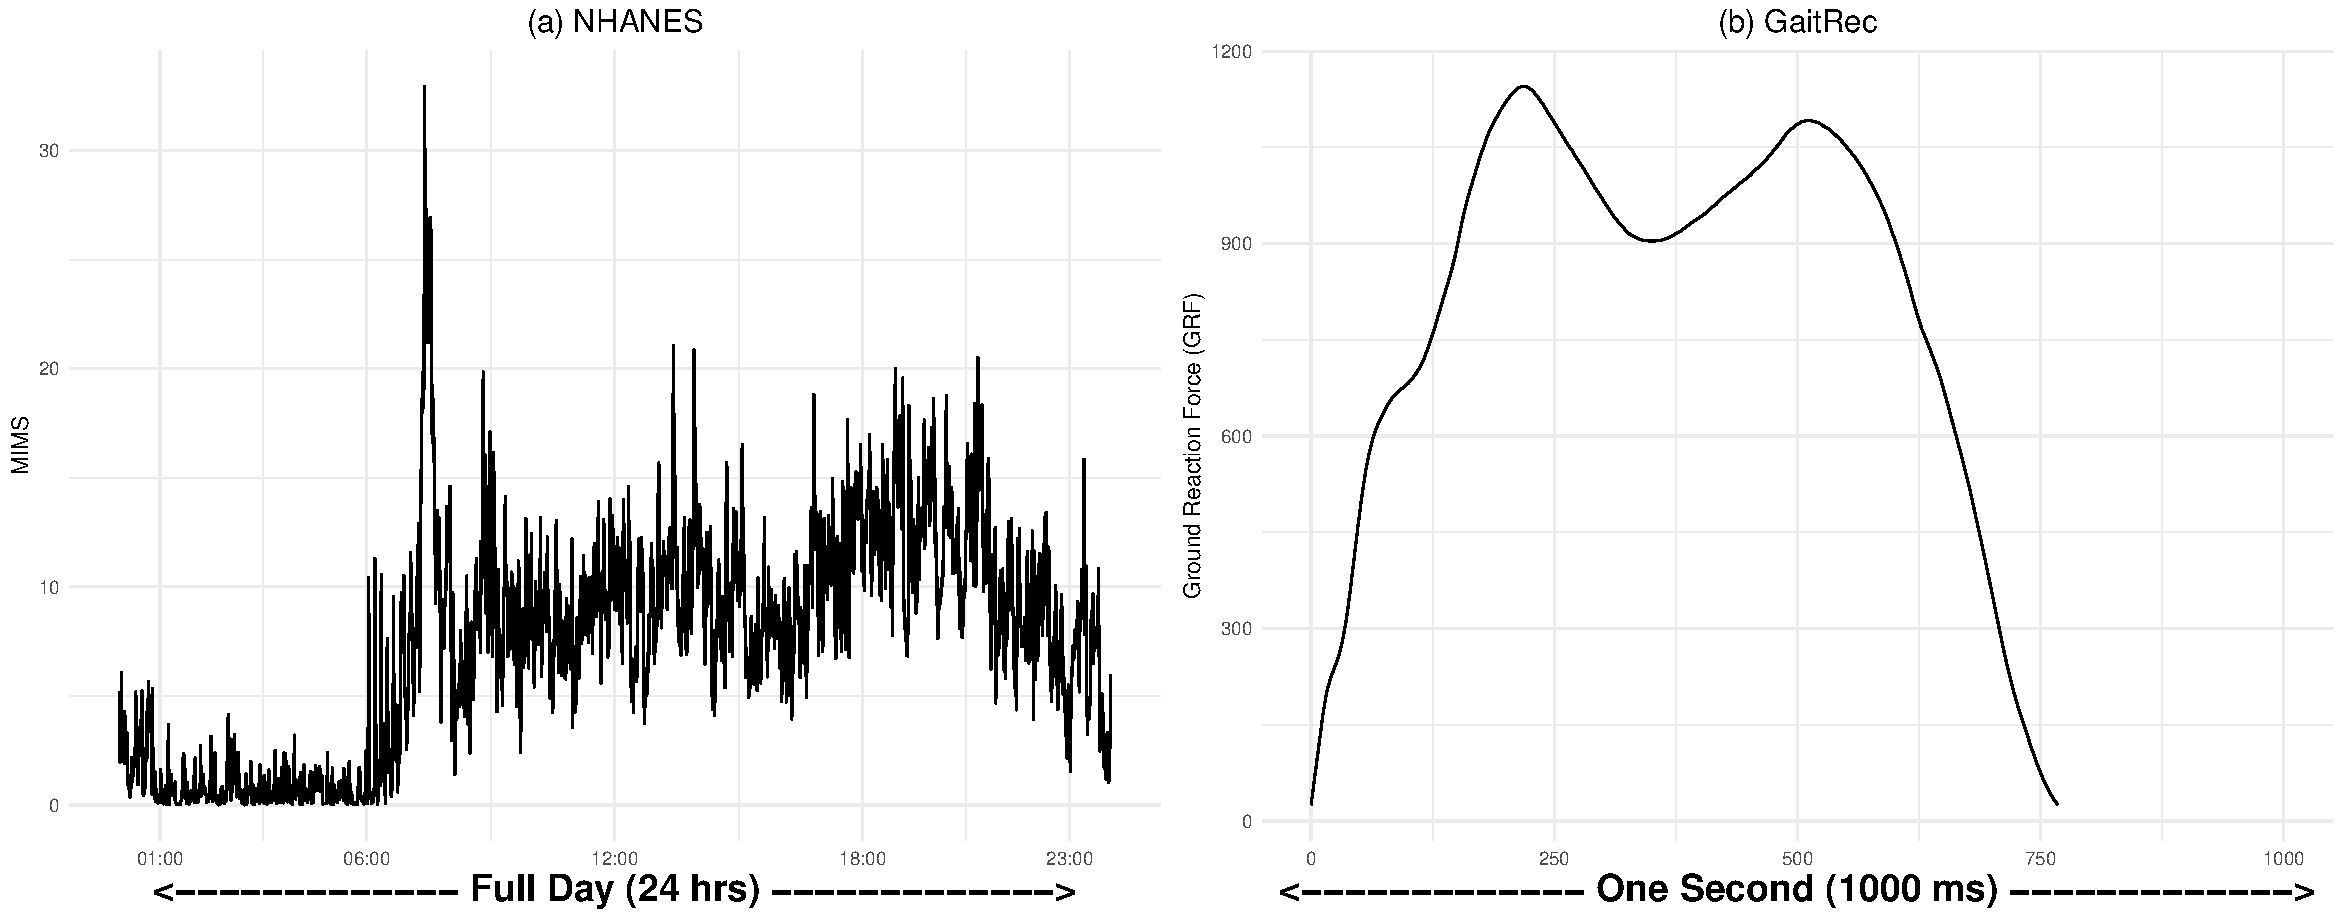
\includegraphics[width=0.6\linewidth]{figures/PA-vs-mocap.pdf}
        \small
        \caption{\textbf{(a)} NHANES \parencite{crainiceanu_functional_2024}; \textbf{(b)} GaitRec \parencite{horsak_gaitrec_2020}.}
        \label{fig:enter-label}
    \end{figure}

    \begin{columns}[c]
    \small
    \column{.45\textwidth}
    \pause \textbf{Differences}:
    \begin{itemize}
        \pause \item Movement on macro vs. micro scales.
        \pause \item Smoothness/ SNR ratios (within and between).
    \end{itemize}
    \column{.5\textwidth}
    \pause \textbf{Similarities}:
    \begin{itemize}
        \pause \item Complex temporal features (scalar summaries insufficient).
        \pause \item Structured dependence (e.g., multilevel, longitudinal).
    \end{itemize}
    \end{columns}
    \vskip1em
    \pause \emph{$\rightarrow$ We need principled and efficient statistical modelling approaches to extract information from rich, complex and structured functional data.}
\end{frame}

\begin{frame}{GaitRec \parencite{horsak_gaitrec_2020}}

\begin{figure}
    \centering
    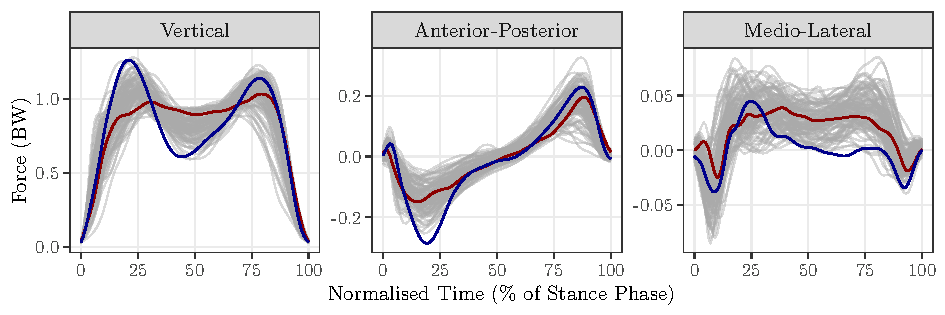
\includegraphics[width=0.8\linewidth]{figures/gaitrec-intro-plot.pdf}
    \caption{A sample of observations from the GaitRec dataset \parencite{horsak_gaitrec_2020}. }
    \label{fig:enter-label}
\end{figure}
\begin{itemize}
    \pause \item Ground reaction force and centre of pressure during walking (kinetics).
    \pause \item 2,295 individuals measured under different conditions (75,732 trials in total).
    \pause \item Healthy controls and individuals with impairments in the hip, knee, ankle and calcaneus.
\end{itemize}
\end{frame}

\begin{frame}{
\includegraphics[width = 0.225 \textwidth]{figures/RISC-logo.pdf} Motivating Dataset}
\centering
\pause \includegraphics[width=1\textwidth]{figures/RISC-Diagram.pdf}    
\end{frame}


\begin{frame}{
\includegraphics[width = 0.225 \textwidth]{figures/RISC-logo.pdf} Motivating Dataset}
    \centering  
    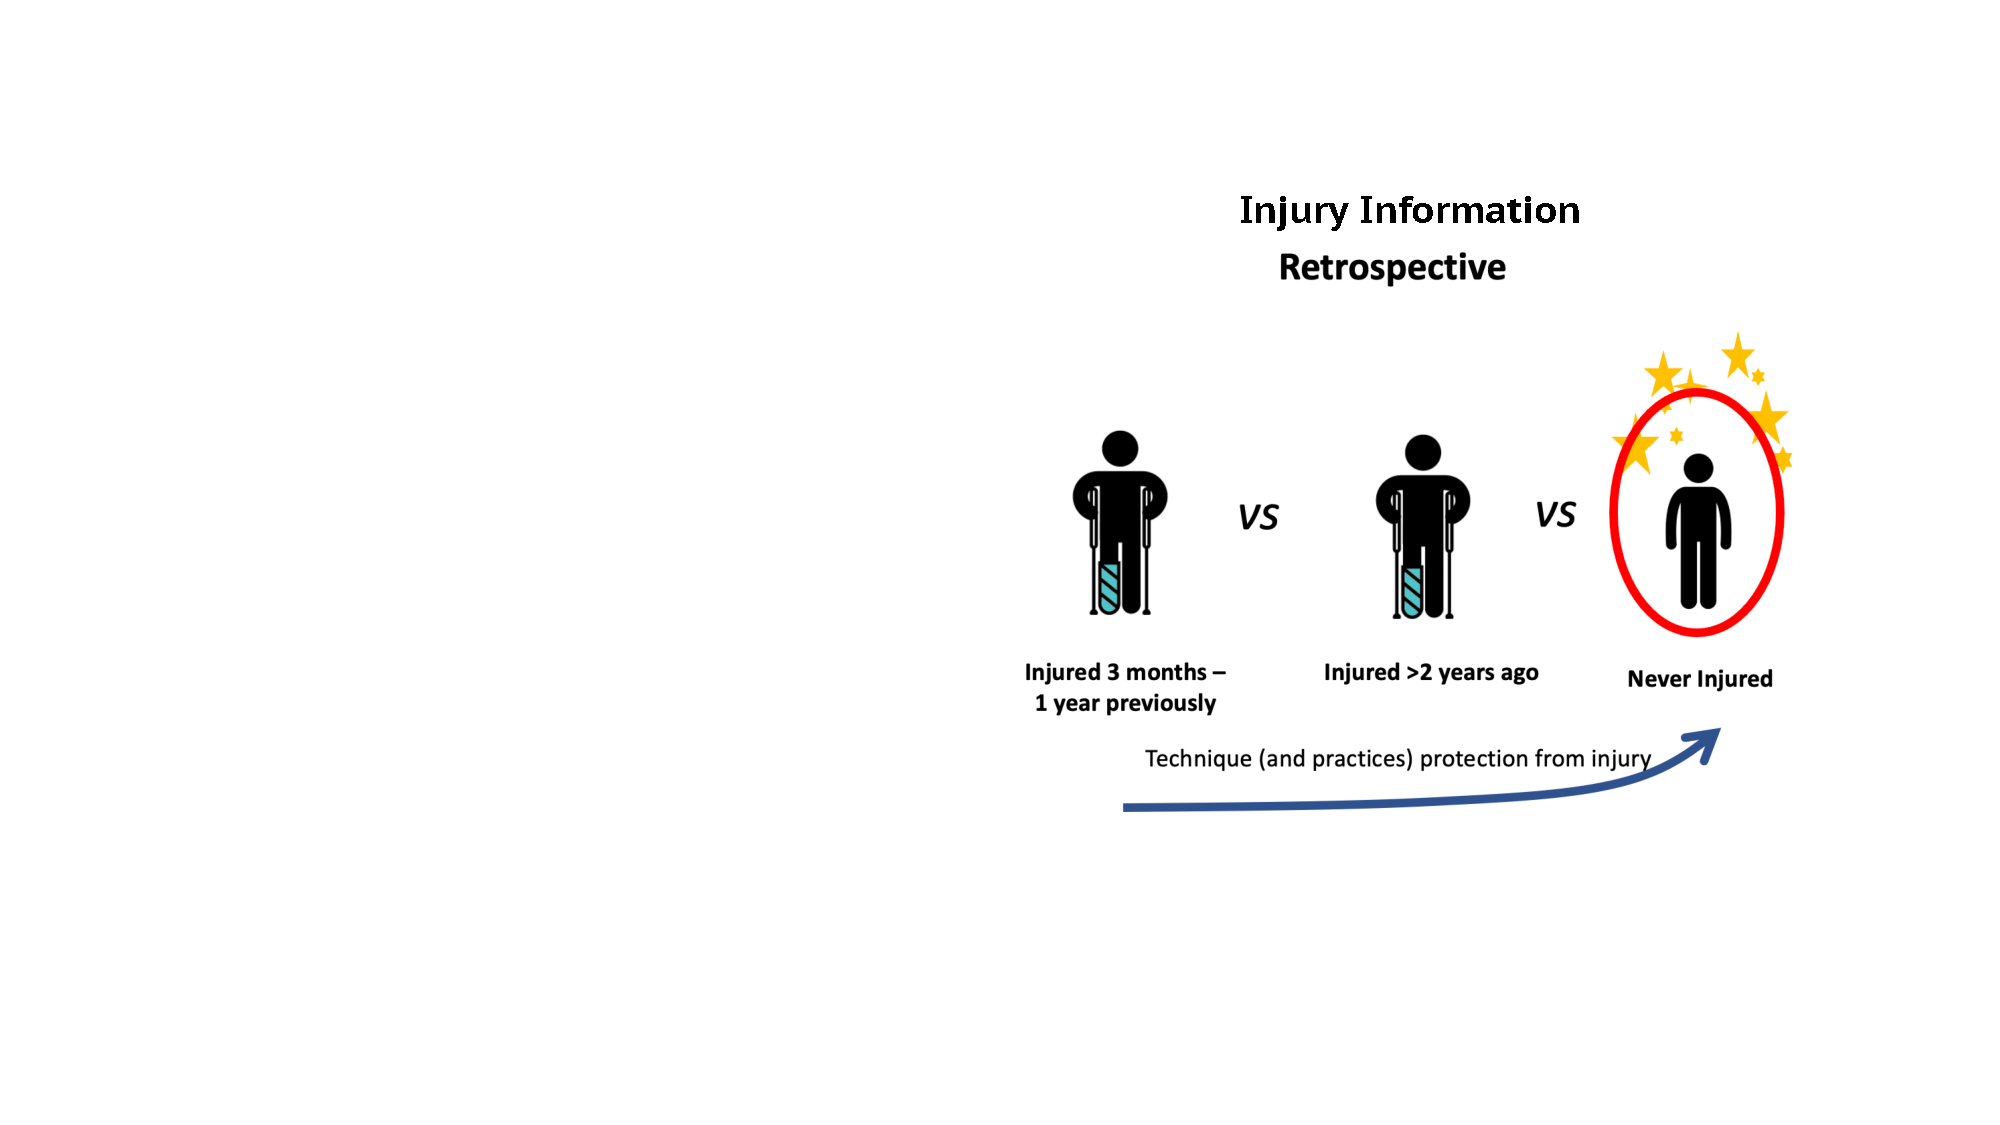
\includegraphics[width = 1\textwidth]{figures/Retro-Injury-Problem-Reduced.pdf}
\end{frame}

\begin{frame}[noframenumbering]{
\includegraphics[width = 0.225 \textwidth]{figures/RISC-logo.pdf} Motivating Dataset}
    \centering  
    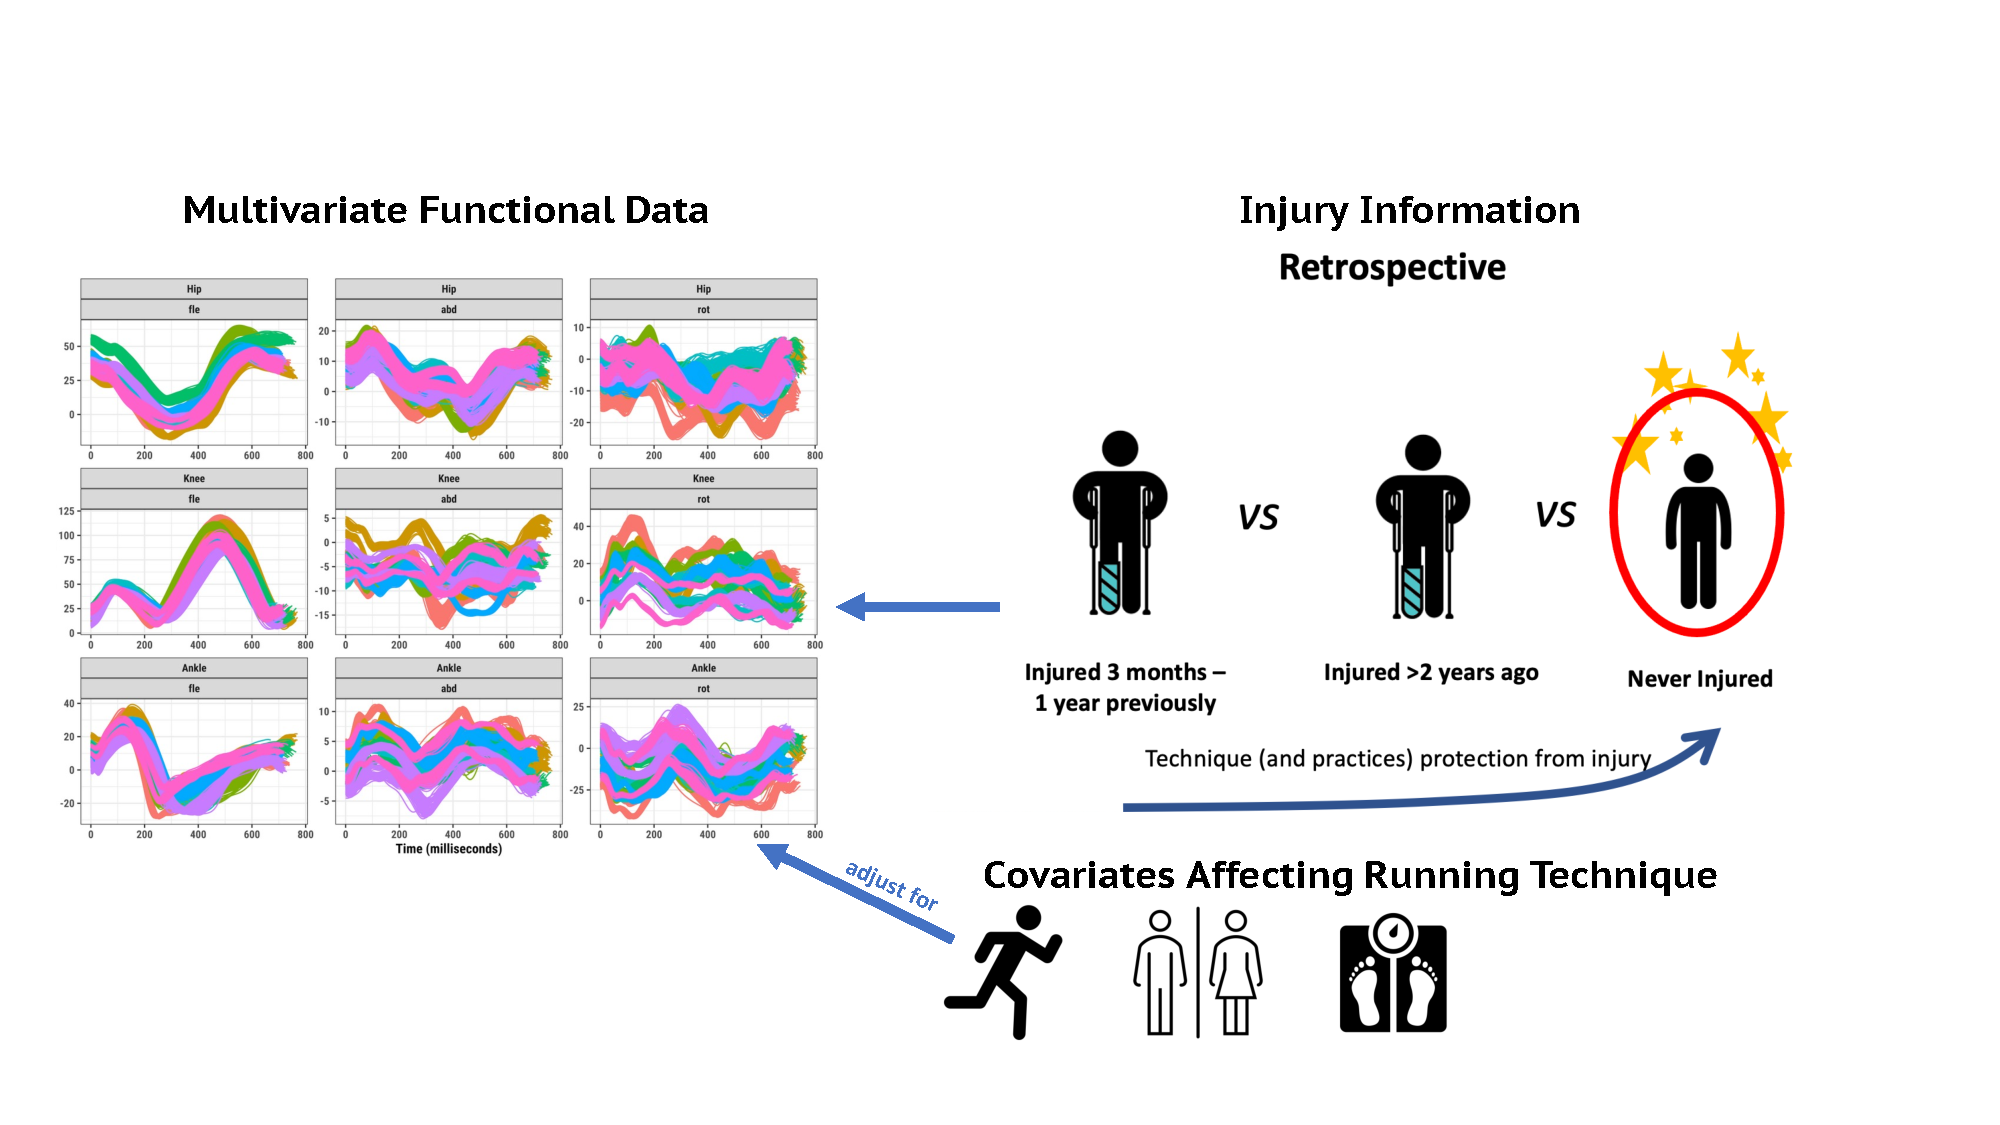
\includegraphics[width = 1\textwidth]{figures/Retro-Injury-Problem-Full.pdf}
\end{frame}


\begin{frame}{Initial Approach \parencite{gunning_analyzing_2023}}
\begin{itemize}
    \pause \item ``Start simple" $\rightarrow$ focus on average bilateral hip and knee flexion angles.
    \pause \item Regress the average bivariate functions on scalar covariates, e.g., injury status, sex, speed \dots
\end{itemize}
\vskip0.5em
\centering
\pause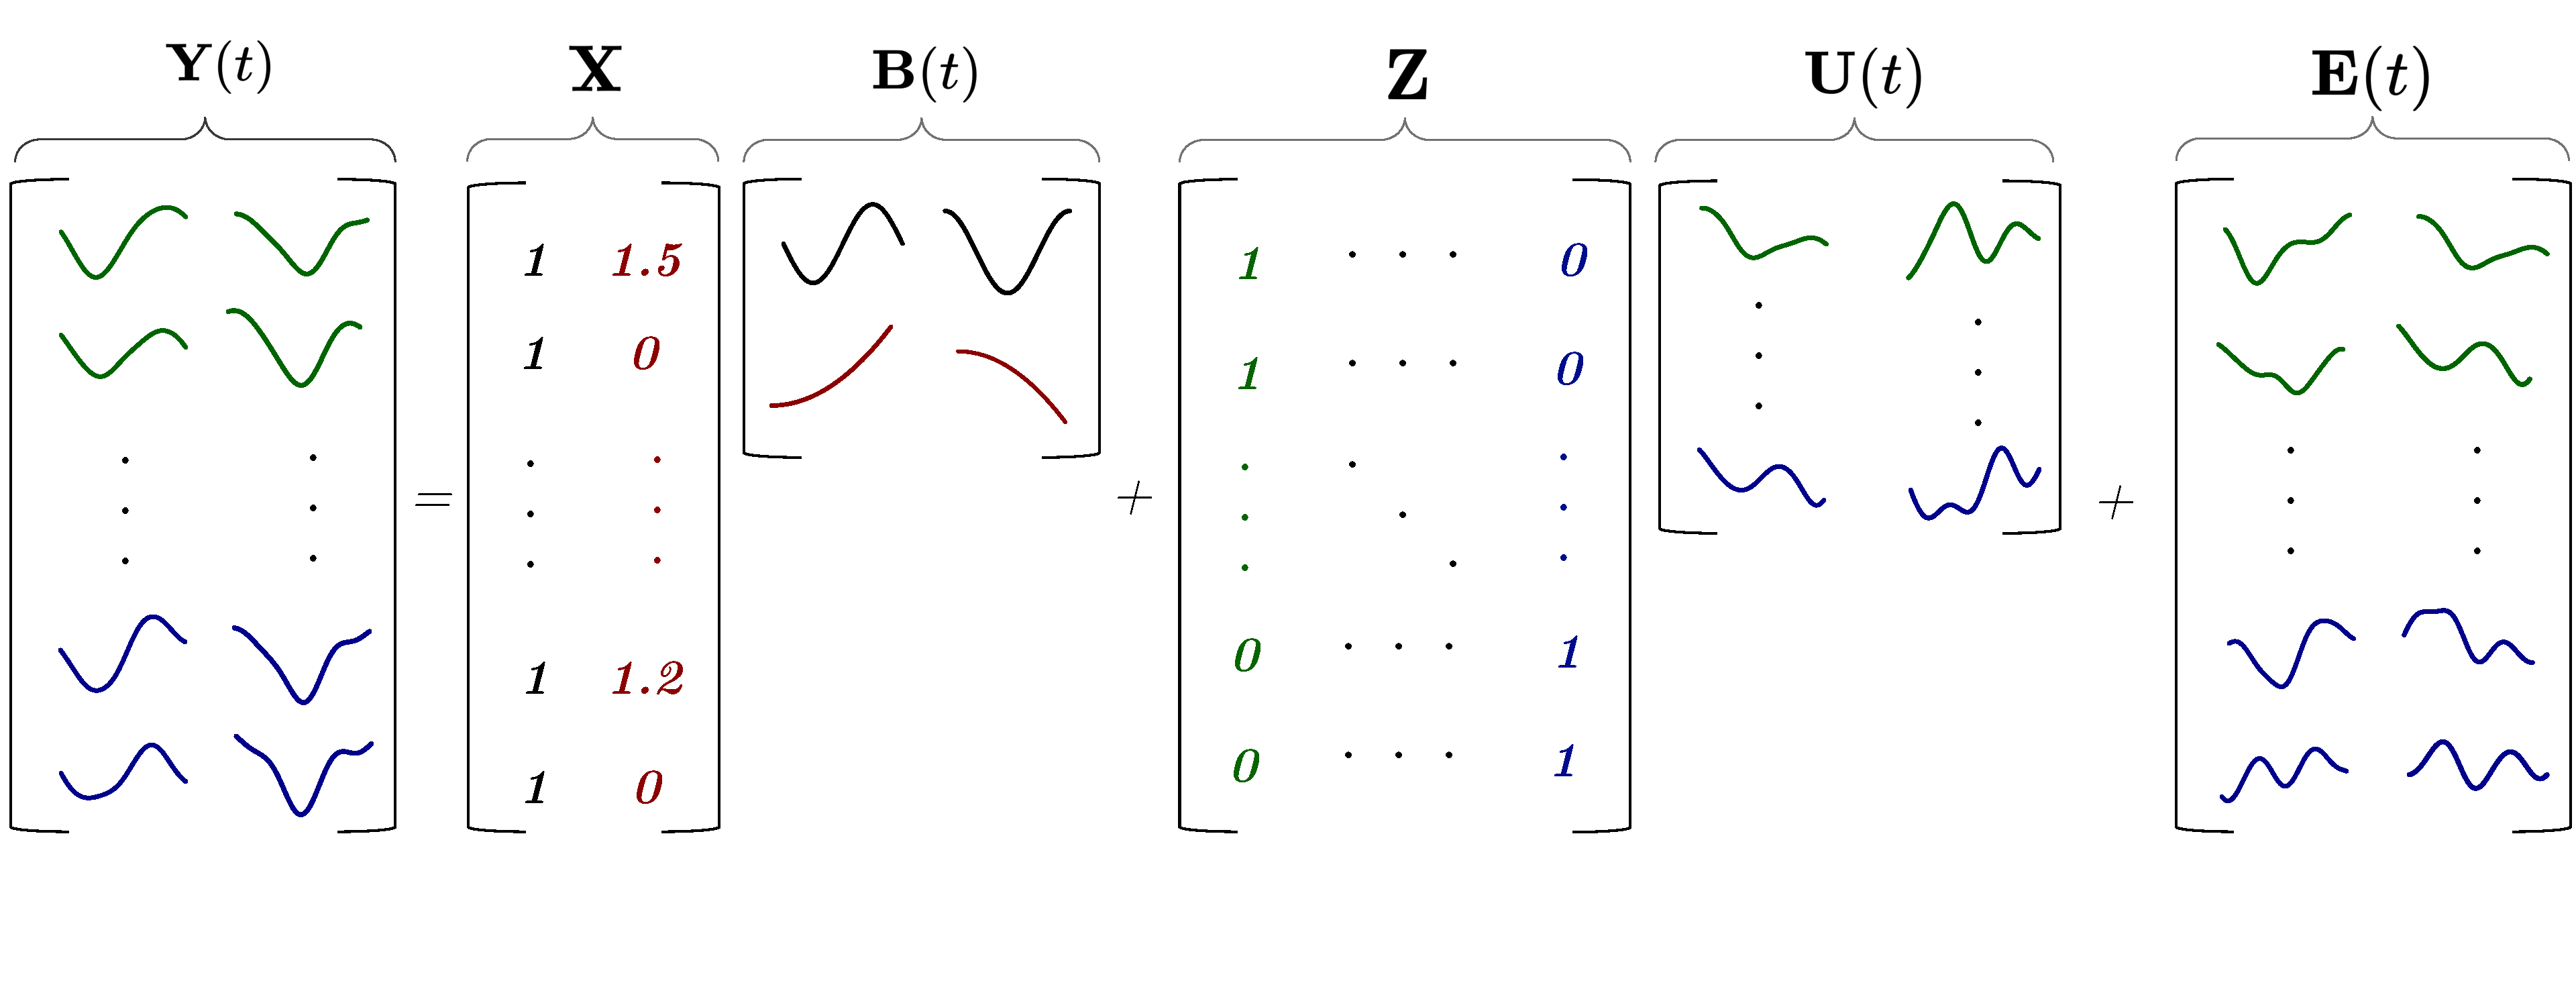
\includegraphics[width = 0.9 \textwidth]{figures/mfmm-diagram.pdf}
\vskip0.5em
% \begin{columns}[c] % The "c" option specifies centered vertical alignment while the "t" option is used for top vertical alignment
%     \centering
%     \column{.5\textwidth} % Left column and width
%     \centering
%     \pause \textbf{Estimation and Inference}
%     \vskip0.5em
%     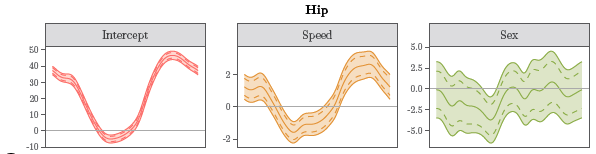
\includegraphics[width = 1\textwidth]{figures/confidence-bands.png}
%     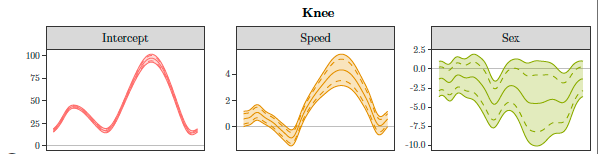
\includegraphics[width = 1 \textwidth]{figures/confidence-bands-02.png}

%     \pause \column{.5\textwidth} % Right column and width
%     \centering
%     \textbf{Covariance Analysis}
%     \vskip0.75em
%     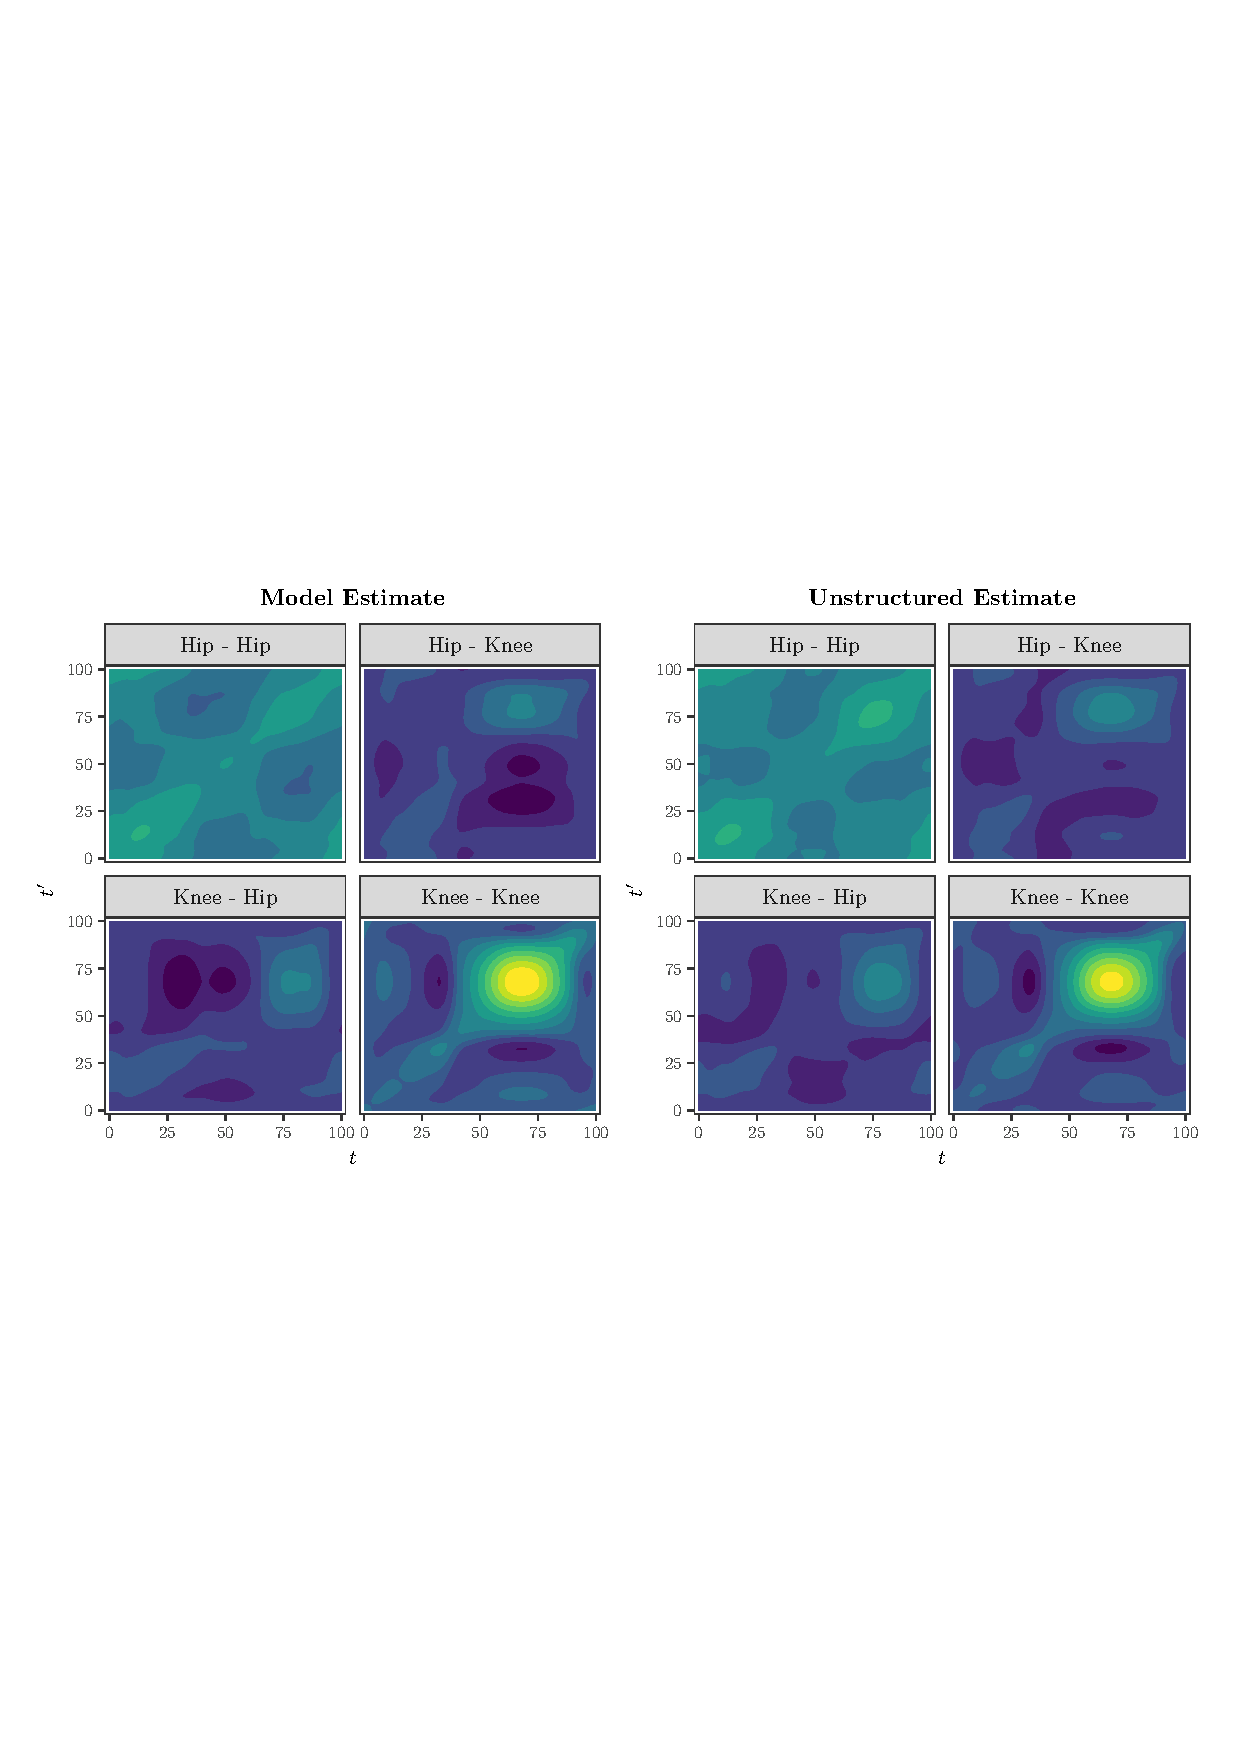
\includegraphics[width = 1\textwidth]{figures/covariance-figure.pdf}
%  \end{columns}
\end{frame}

\begin{frame}{Initial Approach \parencite{gunning_analyzing_2023}}
\begin{itemize}
    \pause \item Developed a simple, flexible and scalable multivariate functional mixed effects modelling approach based on the basis modelling approach of \textcite{morris_wavelet-based_2006}.
\end{itemize}
\pause \begin{figure}
    \centering
    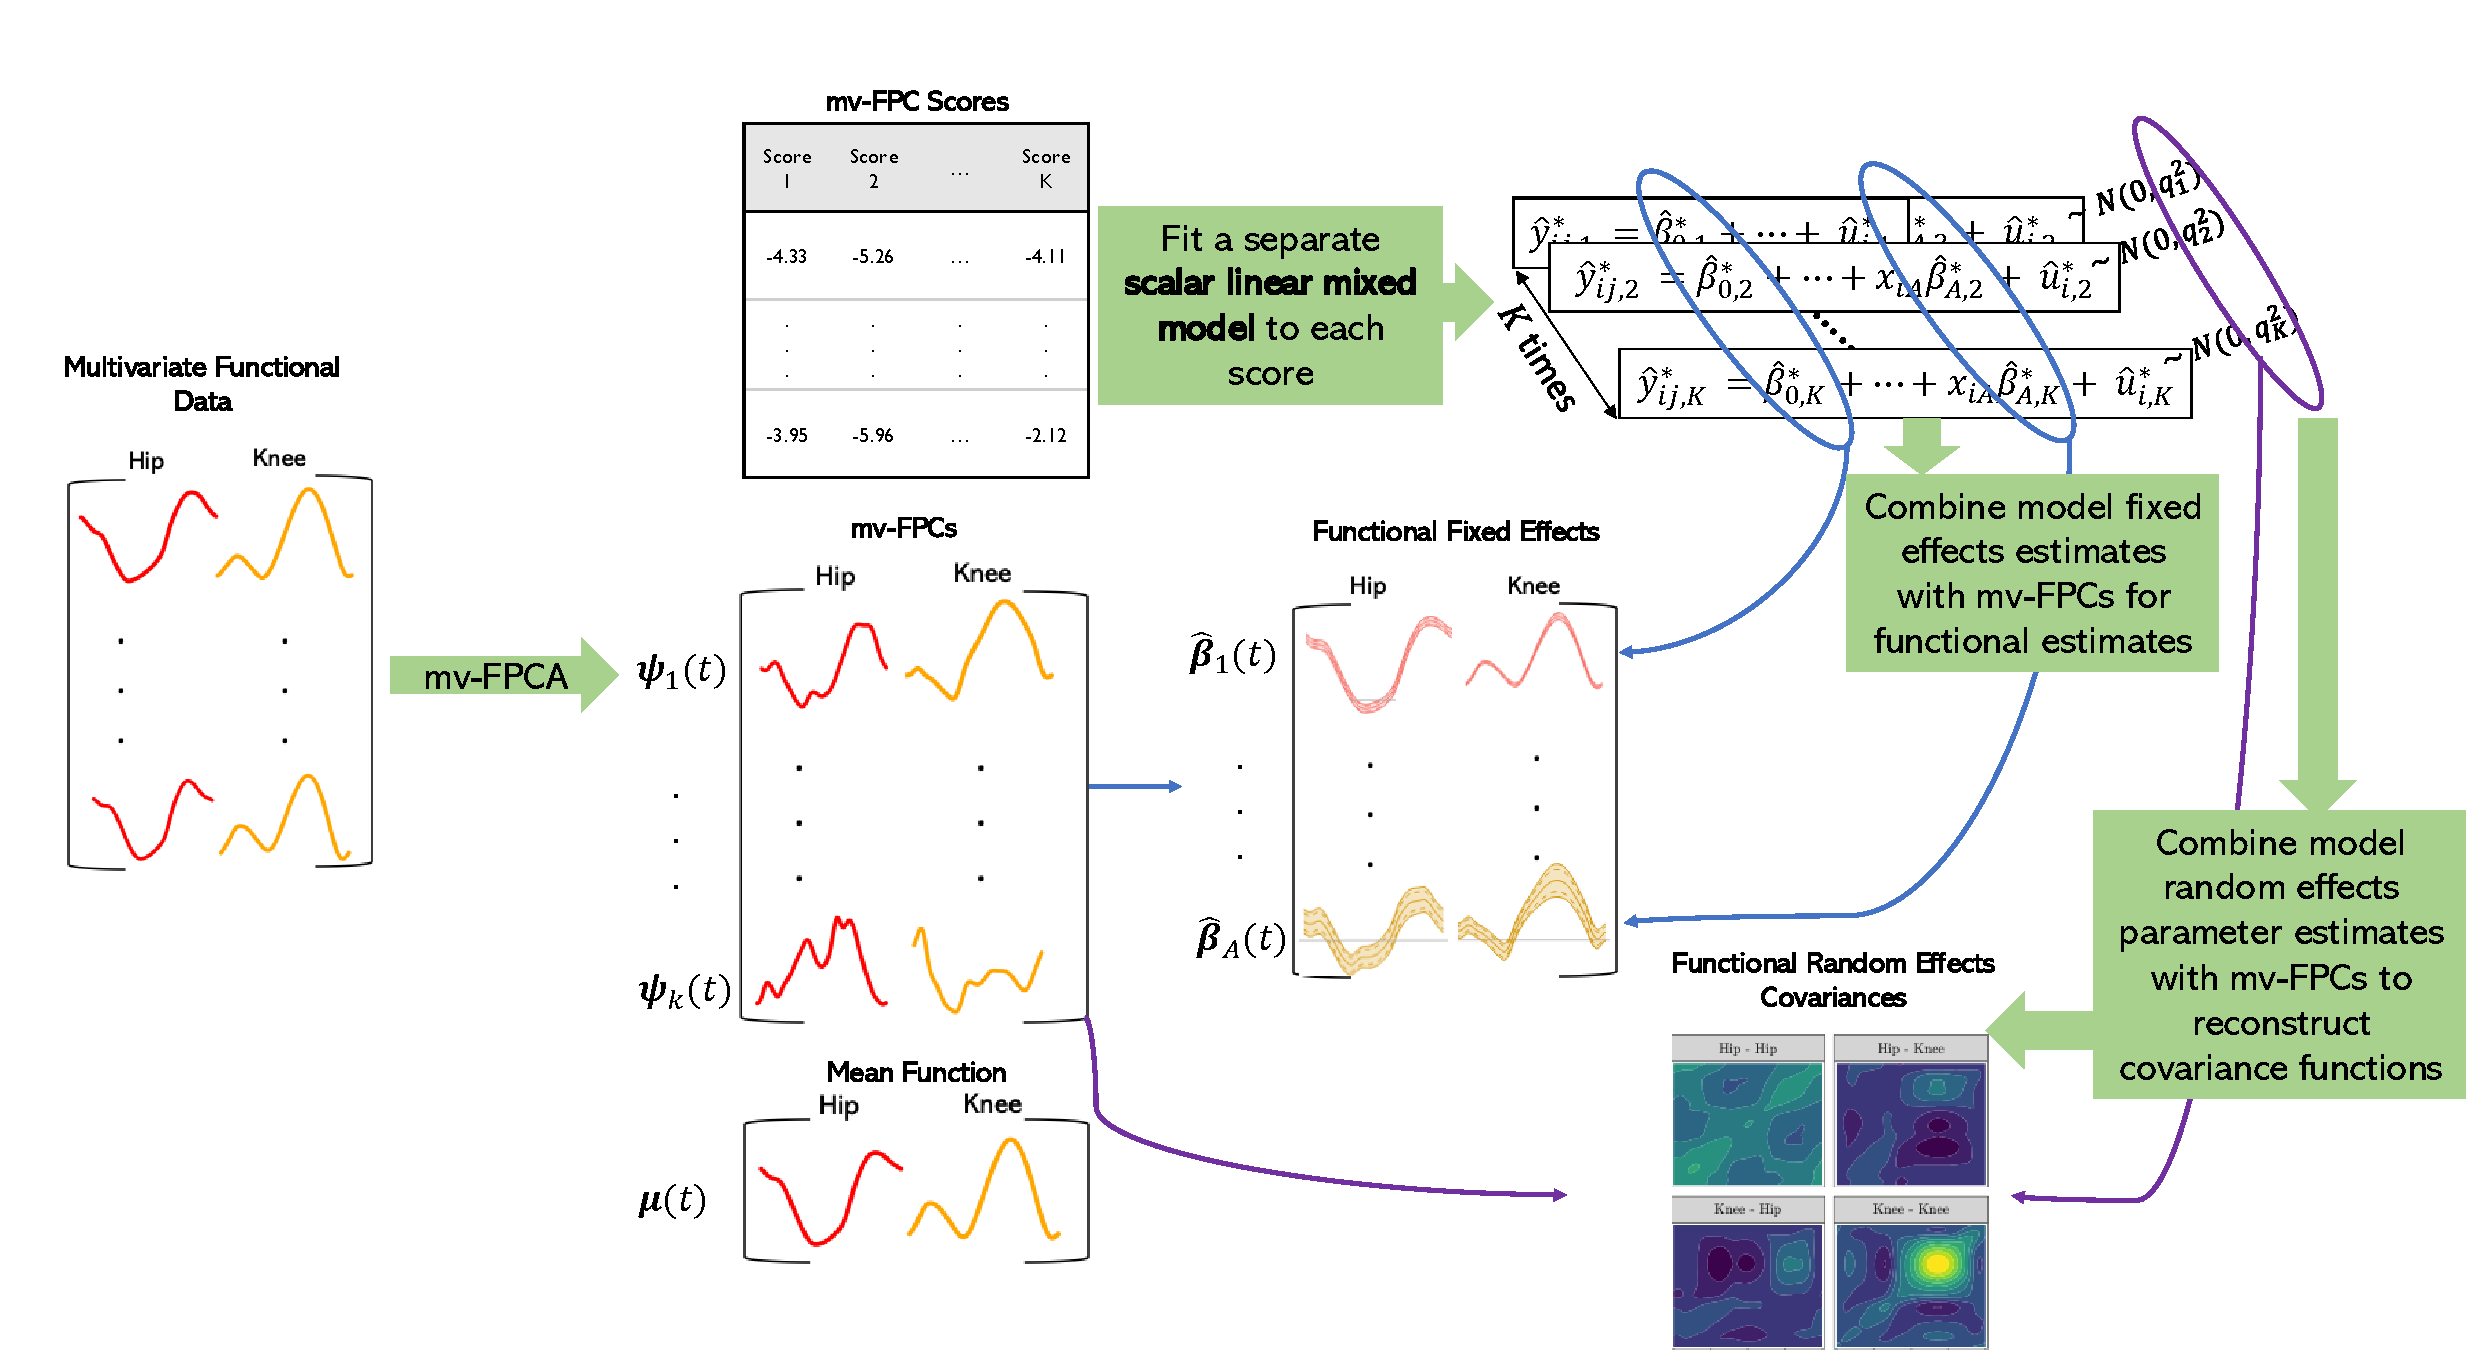
\includegraphics[width=0.75\linewidth]{figures/flowchart.pdf}
    \caption{Flowchart of methodology.}
    \label{fig:enter-label}
\end{figure}
\end{frame}

\begin{frame}{Initial Approach \parencite{gunning_analyzing_2023}}
\begin{columns}[c] % The "c" option specifies centered vertical alignment while the "t" option is used for top vertical alignment
    \centering
    \column{.5\textwidth} % Left column and width
    \centering
    \textbf{Estimation and Inference}
    \vskip0.5em
    \small
    \begin{itemize}
        \item Bayesian approach of \textcite{morris_wavelet-based_2006} uses MCMC for estimation and inference of functional parameters.
        \item We adapt resampling and simulation ideas from \textcite{crainiceanu_bootstrap-based_2012} to implement in a frequentist setting using \texttt{lme4}.
    \end{itemize}
    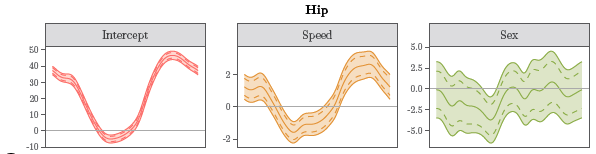
\includegraphics[width = 1\textwidth]{figures/confidence-bands.png}
    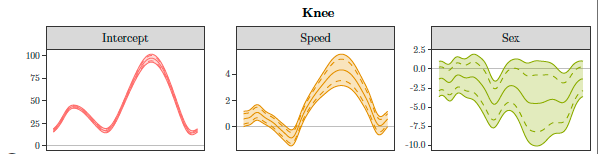
\includegraphics[width = 1 \textwidth]{figures/confidence-bands-02.png}
    \vskip1
    
    \pause \column{.55\textwidth} % Right column and width
    \centering
    \textbf{Covariance Analysis}
    \small
    \begin{itemize}
        \item Modelling each basis coefficient separately makes potentially limiting assumptions on the form of the functional random effects and error covariances.
        \item We propose to check this by using an extension of multilevel FPCA \parencite{di_multilevel_2009} to calculate unstructured estimates to compare with.
    \end{itemize}
    \vskip0.25em
    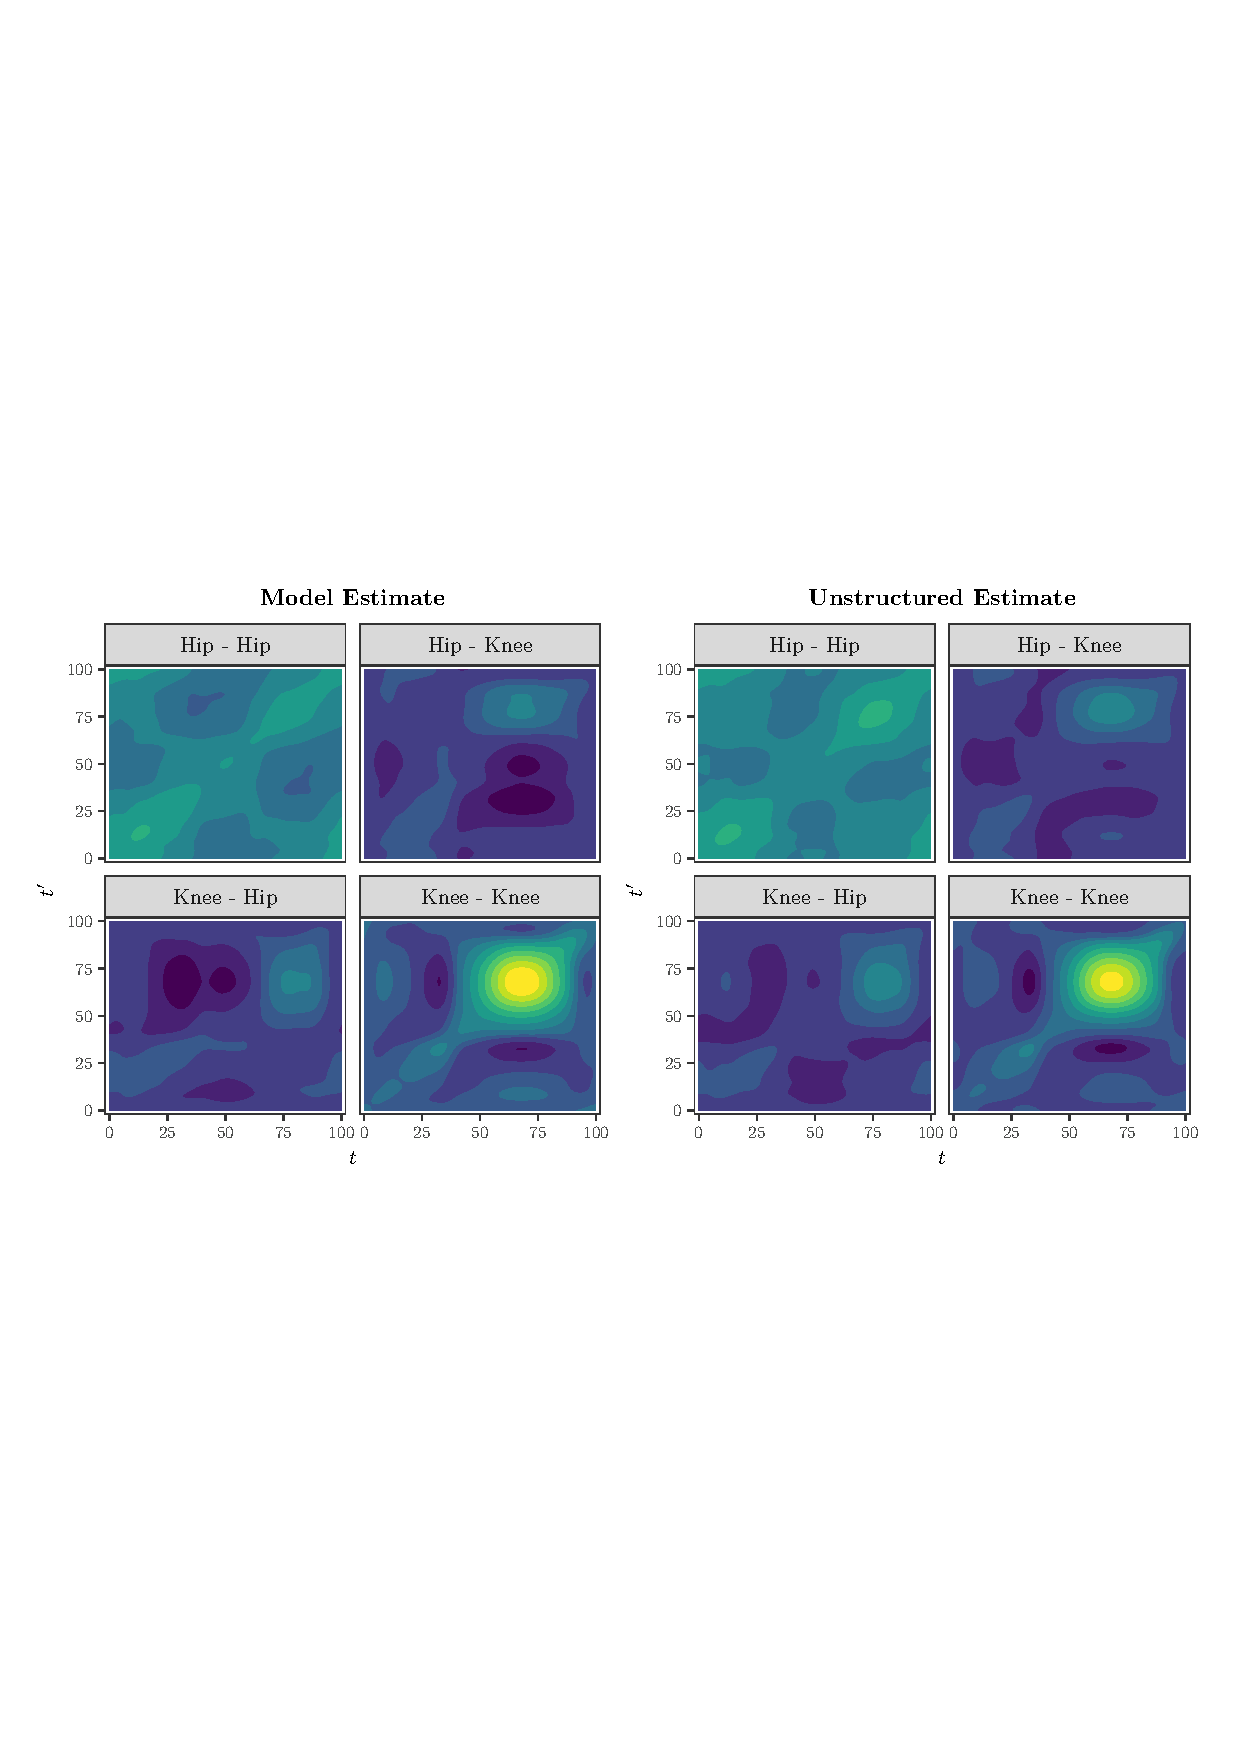
\includegraphics[width = 1\textwidth]{figures/covariance-figure.pdf}
 \end{columns}
\end{frame}

\begin{frame}{Summary and Limitations of Initial Approach}
    \begin{itemize}
        \pause \item Simple methodological approach combines existing methodologies, e.g., \textcite{morris_wavelet-based_2006, di_multilevel_2009, crainiceanu_bootstrap-based_2012}.
        \pause \item Scientific results consistent with and expand upon existing biomechanical literature (e.g., based on scalar values).
        \pause \item \textbf{However, working with an \underline{\textit{average}} stride is potentially wasteful.} For just a one-minute run, this is a data reduction of almost $100:1$.
    \end{itemize}
    \begin{figure}
        \centering
        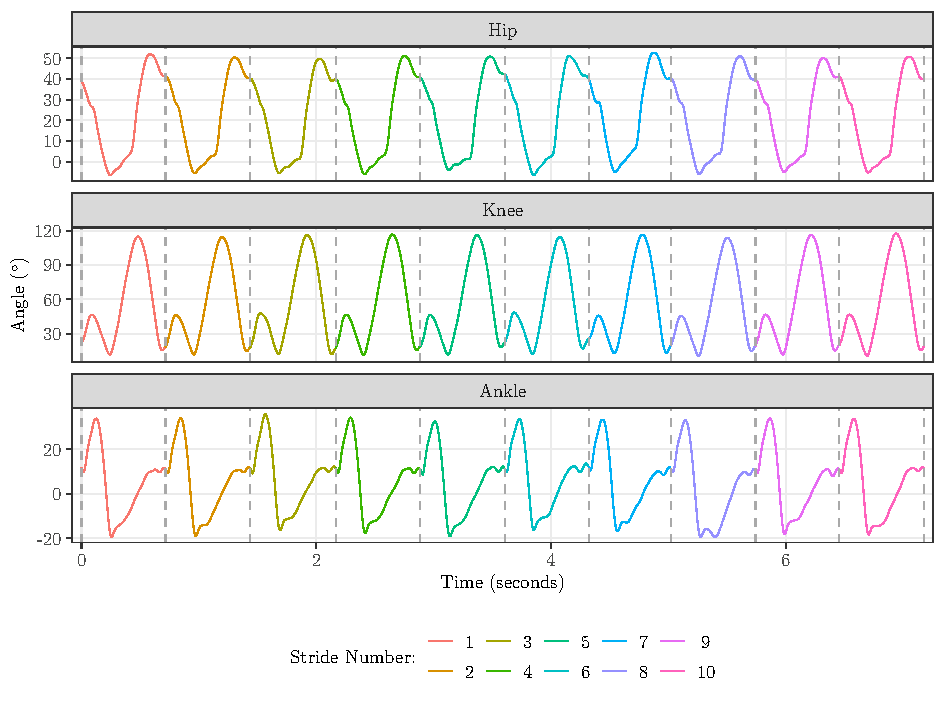
\includegraphics[page = 1, width = 0.5\textwidth]{figures/RISC1-longitudinal-manuscript-code.pdf}
        \caption{The first 10 strides for a single subject.}
        \label{fig:enter-label}
    \end{figure}
\end{frame}

\begin{frame}{Multivariate Multilevel Longitudinal Functional Model \parencite{gunning_multivariate_2023}}
\large
\textbf{Solution}: Develop a structured functional model for \underline{all of the strides}:
\begin{itemize}
    \pause \item Hip, knee and ankle $\rightarrow$ \textbf{multivariate}.
    \pause \item Multiple strides measured bilaterally for each subject $\rightarrow$ \textbf{multilevel}.
    \pause \item Strides have a natural time ordering $\rightarrow$ \textbf{longitudinal}.
\end{itemize}
\end{frame}

\begin{frame}{Multivariate Multilevel Longitudinal Functional Model \parencite{gunning_multivariate_2023}}
Our multivariate multilevel longitudinal functional model is 
$$
\boldy_{ijl} (t) = \boldbeta_0(t, T_{ijl}) + \sum_{a=1}^A x_{ija} \boldbeta_{a} (t) + \mathbf{u}_{i} (t, T_{ijl}) + \mathbf{v}_{ij} (t, T_{ijl}) + \boldsymbol{\varepsilon}_{ijl} (t),
$$
where
\begin{itemize}
\small
    \pause \item $\boldy_{ijl} (t) = \left(y_{ijl}^{(hip)} (t), y_{ijl}^{(knee)} (t), y_{ijl}^{(ankle)} (t)\right)^\top$,
    \pause \item $t \in [0, 100](\%)$ (``functional time") and $T \in [0, 1]$ (``longitudinal time"), and
    \pause \item $l = 1, \dots n_{ij}$, $j \in \{\text{left, right}\}$, and $i = 1, \dots, N$.
\end{itemize}
\end{frame}

\begin{frame}[noframenumbering]{Multivariate Multilevel Longitudinal Functional Model \parencite{gunning_multivariate_2023}}
Our multivariate multilevel longitudinal functional model is 
$$
\boldy_{ijl} (t) = \underbrace{\boldbeta_0(t, T_{ijl})}_{\text{Intercept}} + \sum_{a=1}^A x_{ija} \boldbeta_{a} (t) + \mathbf{u}_{i} (t, T_{ijl}) + \mathbf{v}_{ij} (t, T_{ijl}) + \boldsymbol{\varepsilon}_{ijl} (t),
$$
where
\begin{itemize}
\small
    \item $\boldy_{ijl} (t) = \left(y_{ijl}^{(hip)} (t), y_{ijl}^{(knee)} (t), y_{ijl}^{(ankle)} (t)\right)^\top$,
    \item $t \in [0, 100](\%)$ (``functional time") and $T \in [0, 1]$ (``longitudinal time"), and
    \item $l = 1, \dots n_{ij}$, $j \in \{\text{left, right}\}$, and $i = 1, \dots, N$.
\end{itemize}
\end{frame}

\begin{frame}[noframenumbering]{Multivariate Multilevel Longitudinal Functional Model \parencite{gunning_multivariate_2023}}
Our multivariate multilevel longitudinal functional model is 
$$
\boldy_{ijl} (t) = \boldbeta_0(t, T_{ijl}) + \underbrace{\sum_{a=1}^A x_{ija} \boldbeta_{a} (t)}_{\text{Fixed Effects}} + \mathbf{u}_{i} (t, T_{ijl}) + \mathbf{v}_{ij} (t, T_{ijl}) + \boldsymbol{\varepsilon}_{ijl} (t),
$$
where
\begin{itemize}
\small
    \item $\boldy_{ijl} (t) = \left(y_{ijl}^{(hip)} (t), y_{ijl}^{(knee)} (t), y_{ijl}^{(ankle)} (t)\right)^\top$,
    \item $t \in [0, 100](\%)$ (``functional time") and $T \in [0, 1]$ (``longitudinal time"), and
    \item $l = 1, \dots n_{ij}$, $j \in \{\text{left, right}\}$, and $i = 1, \dots, N$.
\end{itemize}
\end{frame}

\begin{frame}[noframenumbering]{Multivariate Multilevel Longitudinal Functional Model \parencite{gunning_multivariate_2023}}
Our multivariate multilevel longitudinal functional model is 
$$
\boldy_{ijl} (t) = \boldbeta_0(t, T_{ijl}) + \sum_{a=1}^A x_{ija} \boldbeta_{a} (t) + \underbrace{\mathbf{u}_{i} (t, T_{ijl})}_{\text{Subject}} + \mathbf{v}_{ij} (t, T_{ijl}) + \boldsymbol{\varepsilon}_{ijl} (t),
$$
where
\begin{itemize}
\small
    \item $\boldy_{ijl} (t) = \left(y_{ijl}^{(hip)} (t), y_{ijl}^{(knee)} (t), y_{ijl}^{(ankle)} (t)\right)^\top$,
    \item $t \in [0, 100](\%)$ (``functional time") and $T \in [0, 1]$ (``longitudinal time"), and
    \item $l = 1, \dots n_{ij}$, $j \in \{\text{left, right}\}$, and $i = 1, \dots, N$.
\end{itemize}
\end{frame}

\begin{frame}[noframenumbering]{Multivariate Multilevel Longitudinal Functional Model \parencite{gunning_multivariate_2023}}
Our multivariate multilevel longitudinal functional model is 
$$
\boldy_{ijl} (t) = \boldbeta_0(t, T_{ijl}) + \sum_{a=1}^A x_{ija} \boldbeta_{a} (t) + \mathbf{u}_{i} (t, T_{ijl}) + \underbrace{\mathbf{v}_{ij} (t, T_{ijl})}_{\text{Subject \& Side}} + \boldsymbol{\varepsilon}_{ijl} (t),
$$
where
\begin{itemize}
\small
    \item $\boldy_{ijl} (t) = \left(y_{ijl}^{(hip)} (t), y_{ijl}^{(knee)} (t), y_{ijl}^{(ankle)} (t)\right)^\top$,
    \item $t \in [0, 100](\%)$ (``functional time") and $T \in [0, 1]$ (``longitudinal time"), and
    \item $l = 1, \dots n_{ij}$, $j \in \{\text{left, right}\}$, and $i = 1, \dots, N$.
\end{itemize}
\end{frame}

\begin{frame}[noframenumbering]{Multivariate Multilevel Longitudinal Functional Model \parencite{gunning_multivariate_2023}}
Our multivariate multilevel longitudinal functional model is 
$$
\boldy_{ijl} (t) = \boldbeta_0(t, T_{ijl}) + \sum_{a=1}^A x_{ija} \boldbeta_{a} (t) + \mathbf{u}_{i} (t, T_{ijl}) + \mathbf{v}_{ij} (t, T_{ijl}) + \underbrace{\boldsymbol{\varepsilon}_{ijl} (t)}_{\text{Error}},
$$
where
\begin{itemize}
\small
    \item $\boldy_{ijl} (t) = \left(y_{ijl}^{(hip)} (t), y_{ijl}^{(knee)} (t), y_{ijl}^{(ankle)} (t)\right)^\top$,
    \item $t \in [0, 100](\%)$ (``functional time") and $T \in [0, 1]$ (``longitudinal time"), and
    \item $l = 1, \dots n_{ij}$, $j \in \{\text{left, right}\}$, and $i = 1, \dots, N$.
\end{itemize}
\end{frame}


\begin{frame}{Multivariate Multilevel Longitudinal Functional Model \parencite{gunning_multivariate_2023}}
\small
    Again, take a basis modelling approach\footnote{\tiny Similar idea proposed in univariate two-level case by \textcite{park_longitudinal_2015}.} by representing
    $$
\boldy_{ijl}(t) = \sum_{k=1}^K y_{ijl, k}^* \boldpsi_k (t),
$$
where $y_{ijl, k}^*$ are scalar basis coefficients and $\boldpsi_k (t)$ are multivariate basis functions in the \emph{functional direction} (we choose mv-FPCs).
\vskip1em
\pause Reduces the problem to fitting a series of $K$ mixed models of the form:
$$
y^*_{ijl, k} = \beta_{0, k}^* (T_{ijl}) + \sum_{a=1}^A x_{ia} \beta_{a, k}^*  + u_{i, k}^* (T_{ijl}) + v_{ij, k}^* (T_{ijl}) + \varepsilon_{ijl, k}^*,
$$
\pause which is a standard multilevel functional model \parencite{di_multilevel_2009} in the \emph{longitudinal direction}.
\end{frame}

\begin{frame}{Multivariate Multilevel Longitudinal Functional Model \parencite{gunning_multivariate_2023}}
    Again, we use basis expansions, this time in the longitudinal direction:
    {\scriptsize$$
\beta_{0, k}^* (T) = \sum_{d=1}^D \beta_{0, k, d}^* \ \xi_d(T), \quad  u_{i, k}^* (T) = \sum_{d=1}^D u_{i, k, d}^* \ \xi_d (T) \quad \text{and} \quad v_{ij, k}^* (T) = \sum_{d=1}^D v_{ij, k, d}^* \ \xi_d (T).
$$}

\pause \textbf{Question}: Which basis functions should we use for $u_{i, k}^* (T)$ and $v_{ij, k}^* (T)$?

\pause \begin{figure}
    \centering
    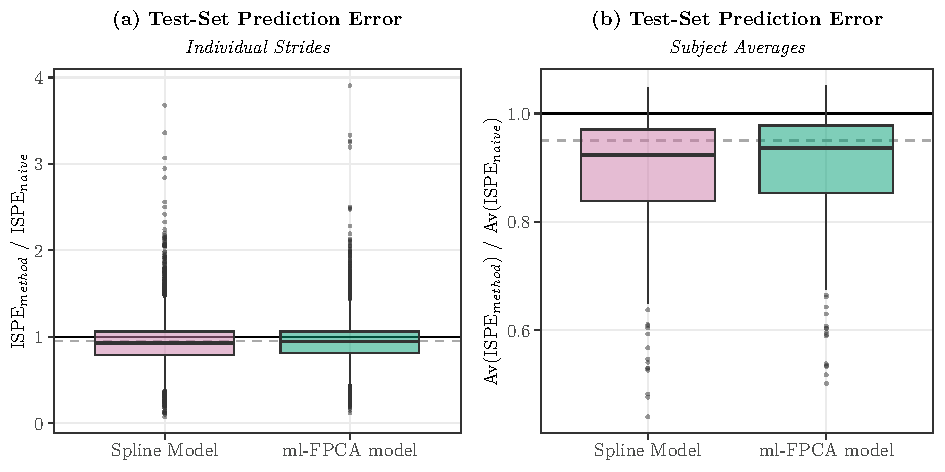
\includegraphics[width=0.6\linewidth]{figures/test-set-PE.pdf}
    \caption{\scriptsize Representation using pre-specified spline (pink) and empirically-determined ml-FPCA basis \parencite[green]{cui_fast_2023} basis functions gives similar results.}
\end{figure}
\end{frame}


\begin{frame}{Results: Fixed Effects}

    \begin{columns}[c]
    \small
    \column{.6\textwidth}
    \begin{itemize}
        \item Fixed effects estimates $$\widehat{\boldbeta}_a(t) = \sum_{k=1}^K \widehat{\beta}_{a, k}^* \boldsymbol{\psi}_k (t).$$
        \item Simultaneous bands account for multiple comparisons across $t$ and the hip, knee and ankle. Obtained using bootstrap and simulation approaches\footnote{\scriptsize See \textcite{faraway_regression_1997, ruppert_semiparametric_2003, crainiceanu_bootstrap-based_2012, park_simple_2018, cui_fast_2022}.}.
        \item Scientific results consistent with existing biomechanical knowledge.
    \end{itemize}
    \column{0.4\textwidth}
    \begin{figure}
    \centering
    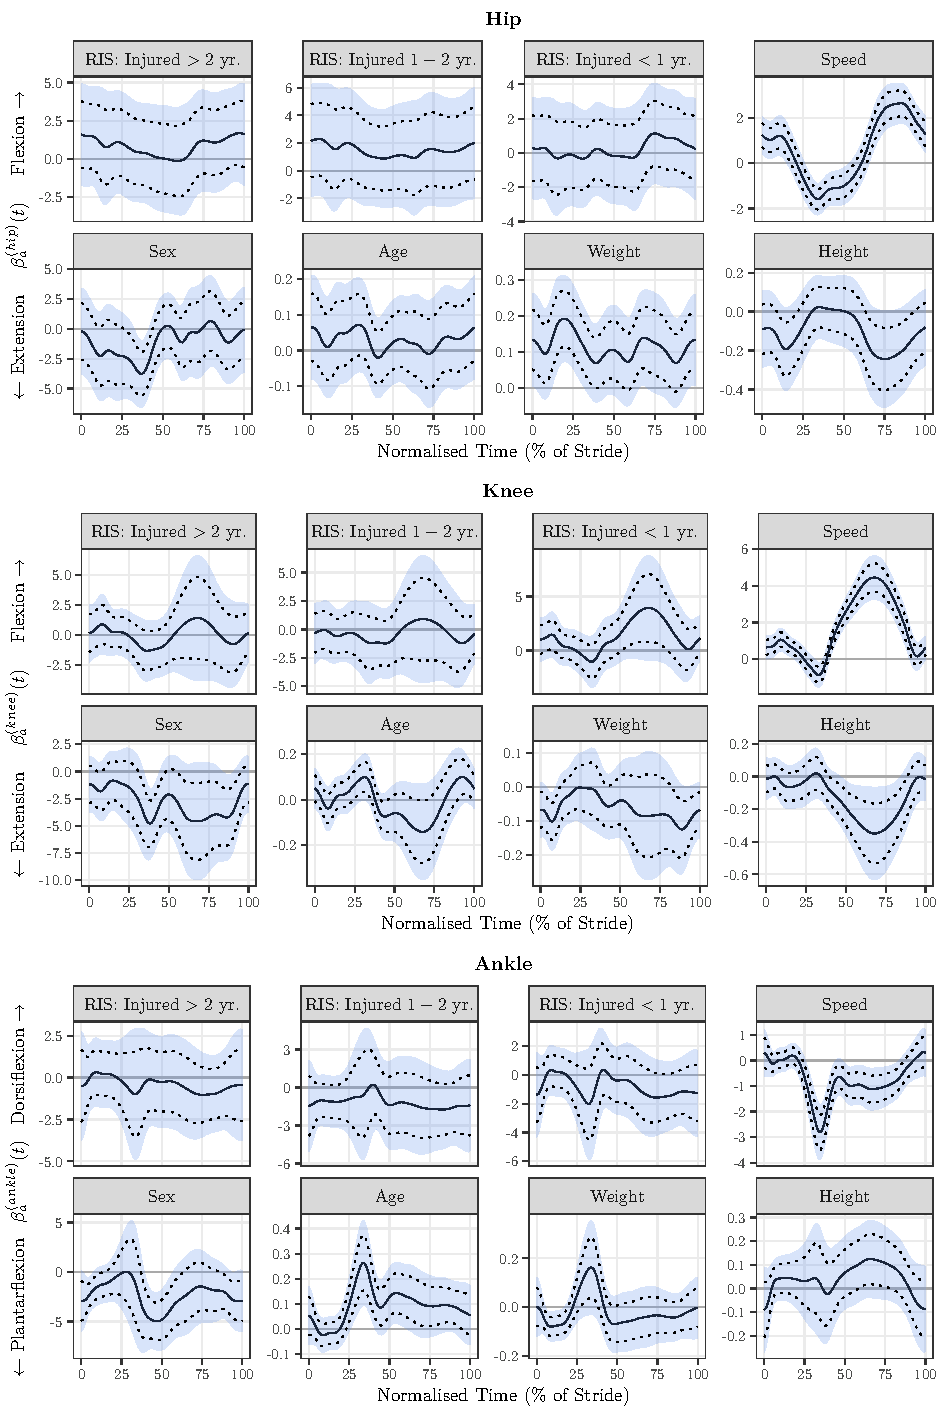
\includegraphics[width=1\linewidth]{figures/fixef_coef_plot.pdf}
    % \caption{Results for }
    % \label{fig:enter-label}
\end{figure}
    \end{columns}
\end{frame}

\begin{frame}{Results: Random Effects}
    Rates of change of $\widehat{\mathbf{u}}_i (t, T)$ and $\widehat{\mathbf{v}}_{ij} (t, T)$ w.r.t. $T$ characterise changes over the course of the treadmill run.
    \vskip2.5em
    \begin{columns}[c]
    \column{.5\textwidth}
    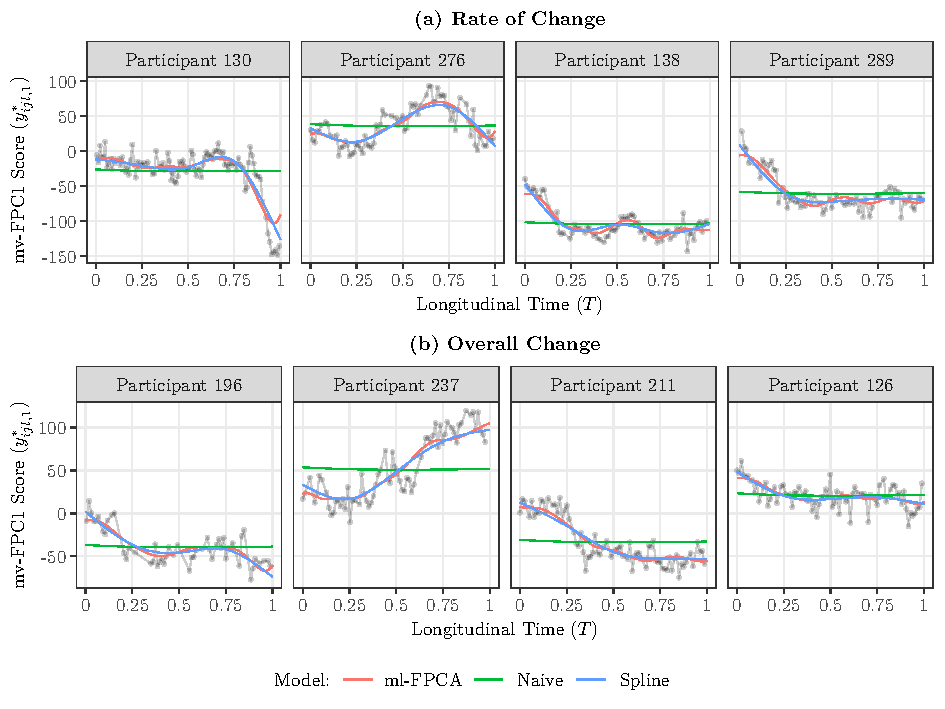
\includegraphics[width = 1\textwidth]{figures/change-plot.pdf}
    \column{.5\textwidth}
    \pause 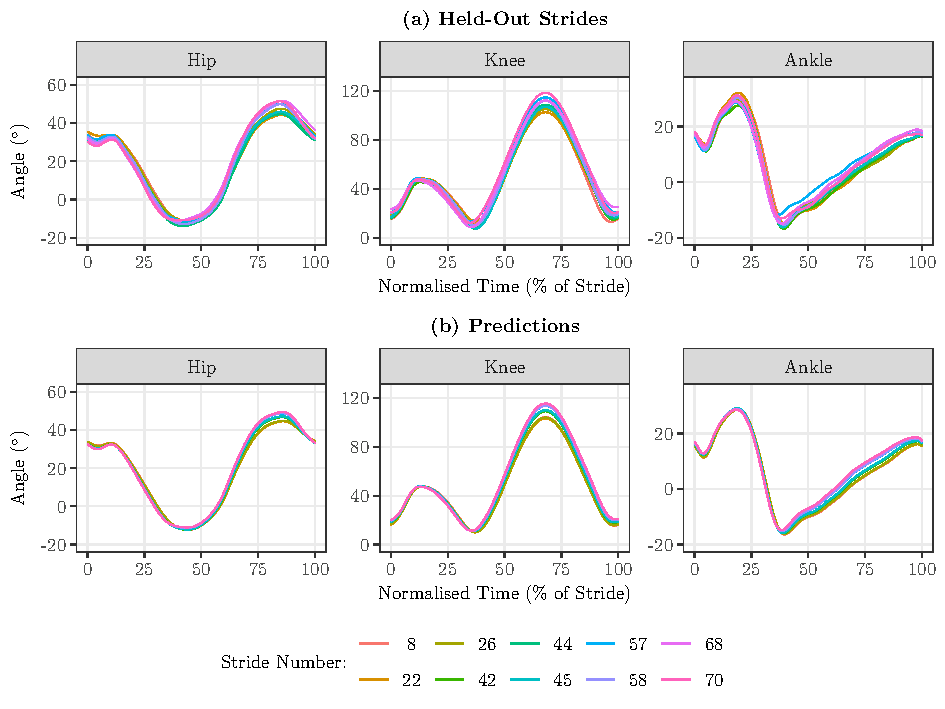
\includegraphics[width = 1\textwidth]{figures/p4237-plot.pdf}
    \end{columns}
\end{frame}

\begin{frame}[noframenumbering]{Results: Random Effects}
    Rates of change of $\widehat{\mathbf{u}}_i (t, T)$ and $\widehat{\mathbf{v}}_{ij} (t, T)$ w.r.t. $T$ characterise changes over the course of the treadmill run.
    \vskip2.5em
    \begin{columns}[c]
    \column{.5\textwidth}
    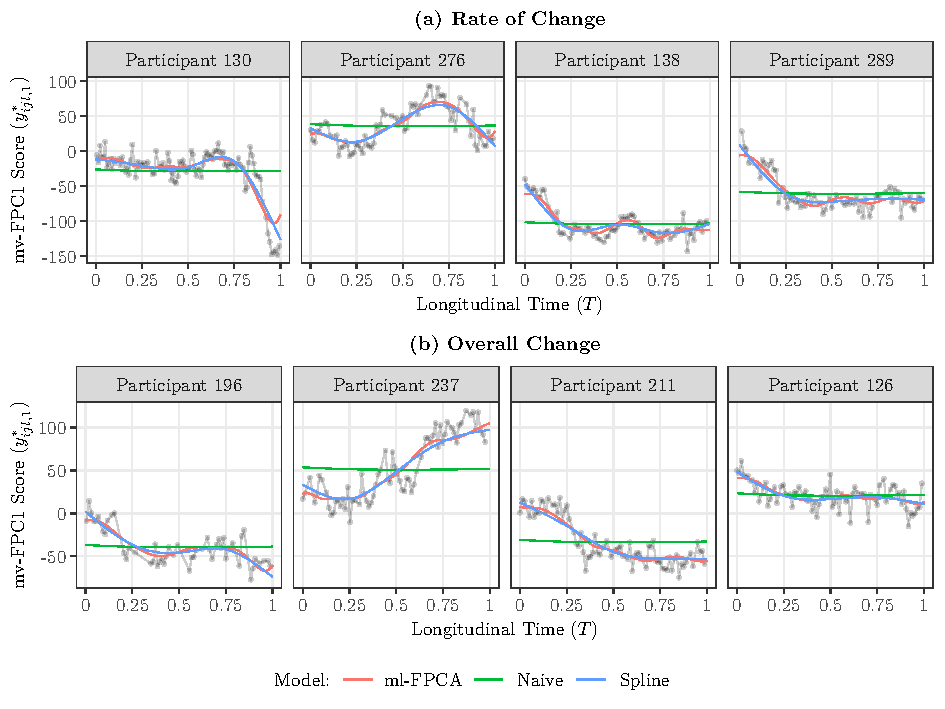
\includegraphics[width = 1\textwidth]{figures/change-plot.pdf}

    \column{.5\textwidth}
    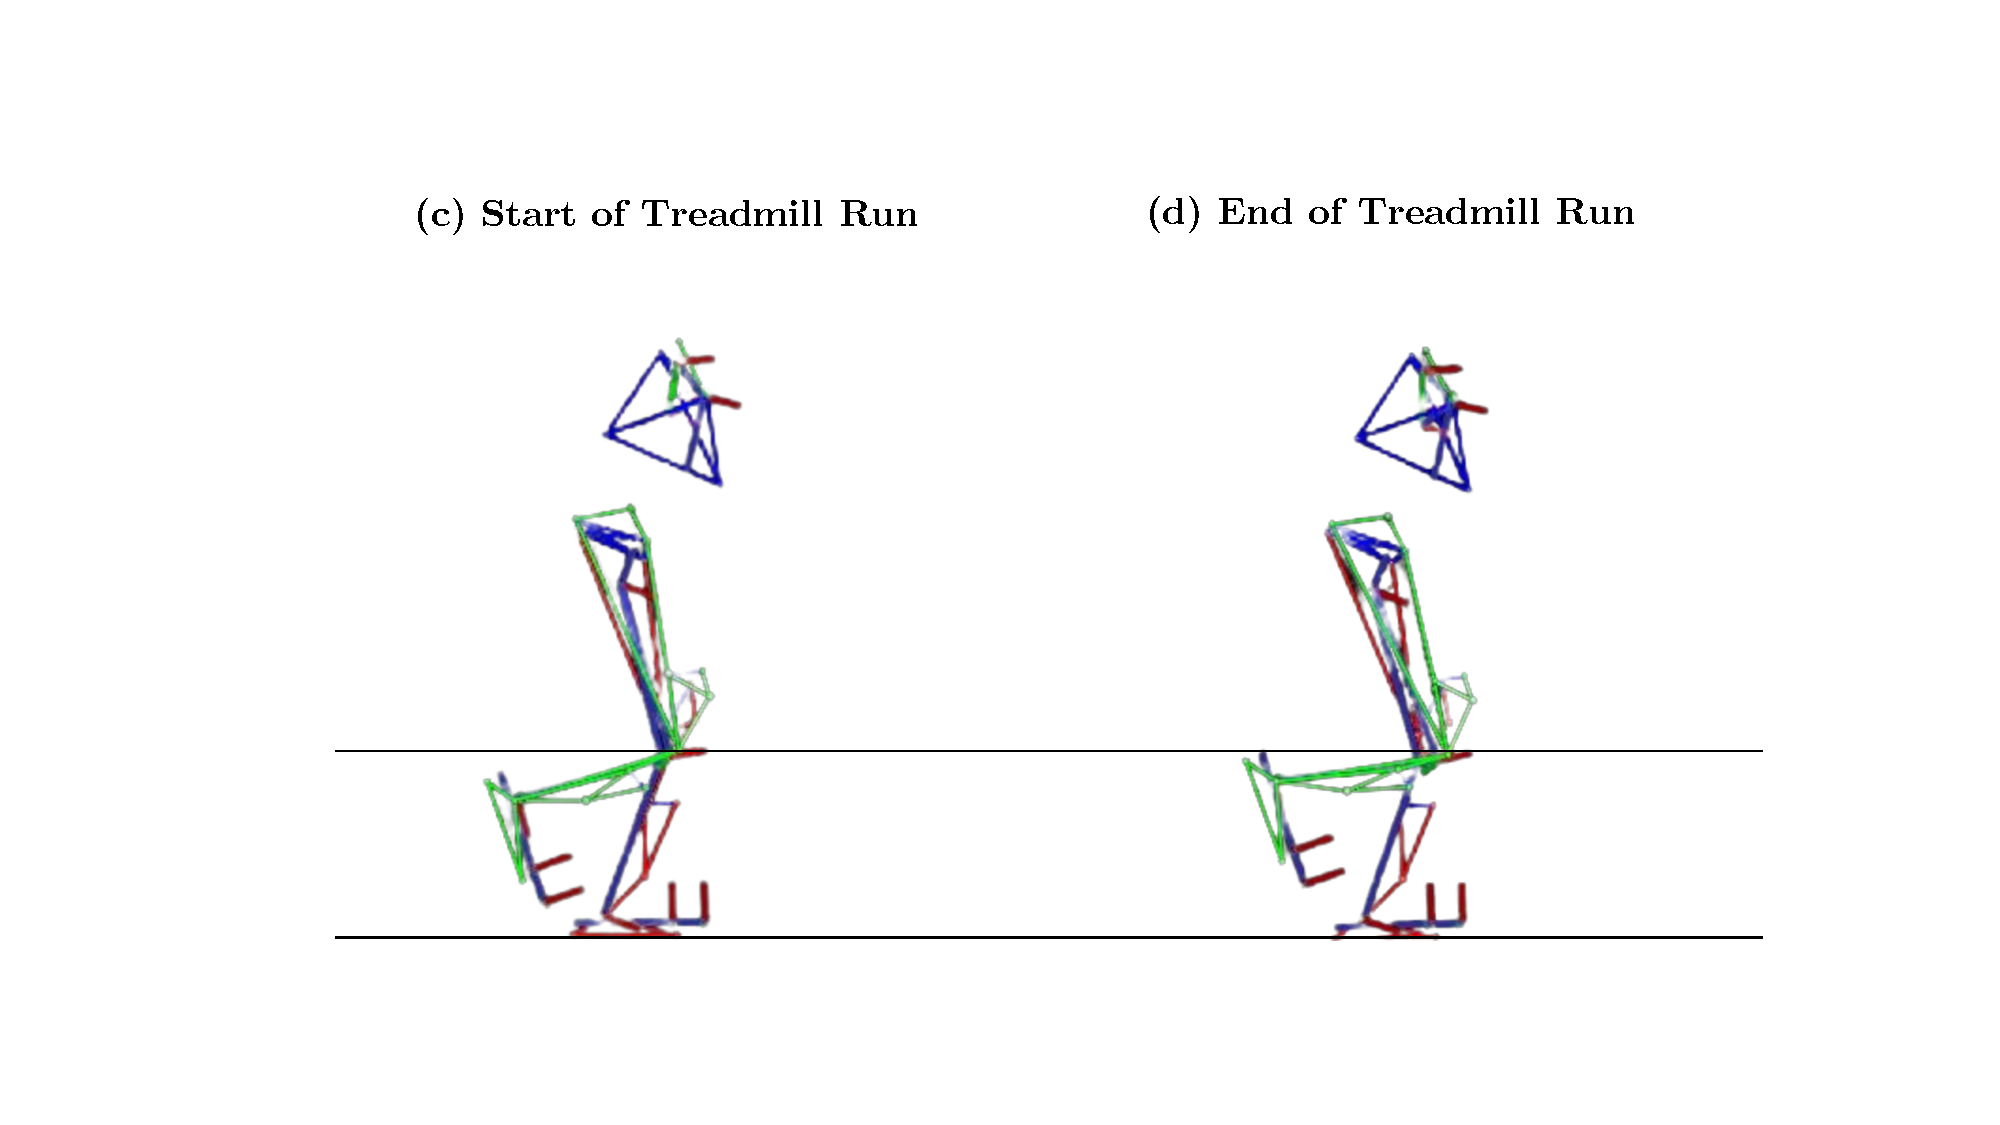
\includegraphics[width = 1\textwidth]{figures/mocap-pic.pdf}
    \end{columns}
\end{frame}

\begin{frame}{Summary}
\begin{itemize}
    \pause \item Simple and flexible approach for modelling streams of smooth multivariate functional data that arise in biomechanics.
    \pause \item Characterise population-level fixed effects and intra-individual longitudinal changes during the treadmill run -- practically meaningful insights.
    \pause \item Potential to use the model in different contexts and extend it to more complex settings -- we are only ``scratching the surface".
\end{itemize}
\begin{figure}
    \centering
    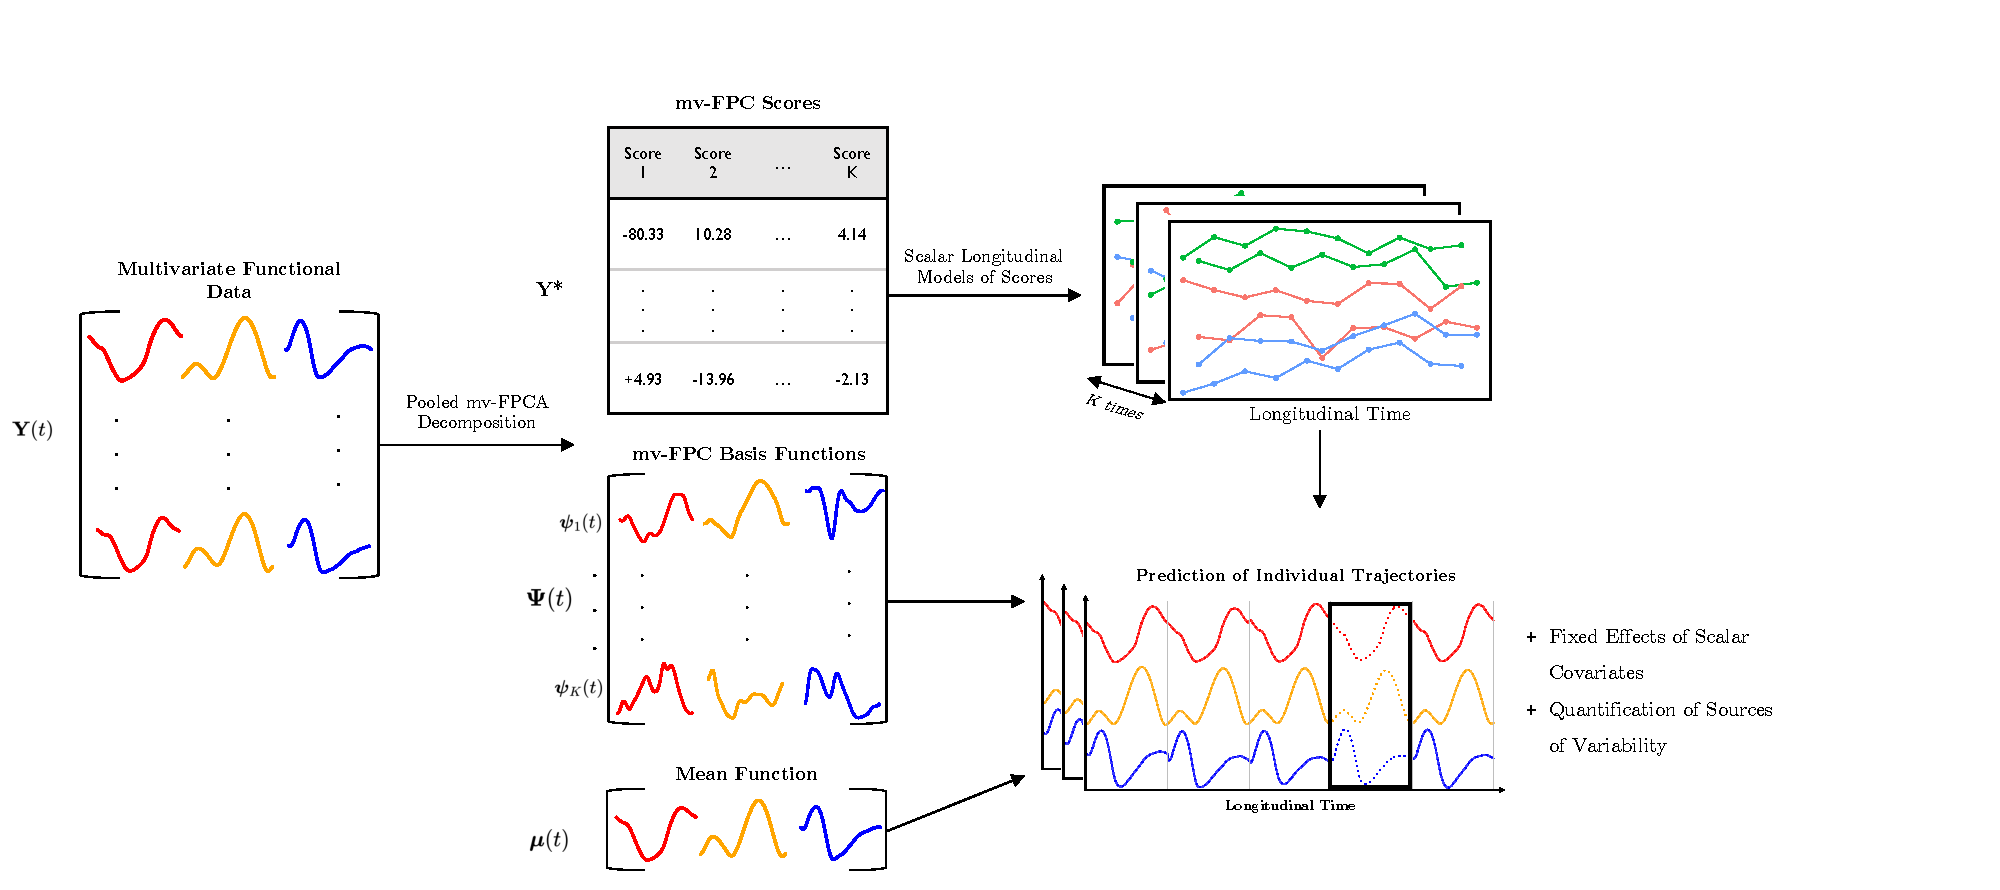
\includegraphics[width=0.65\linewidth]{methods-schematic.pdf}
    \caption{Summary of the modelling approach.}
    \label{fig:enter-label}
\end{figure}
\end{frame}

\begin{frame}
    \vfill
    \Huge{\centerline{\textbf{Thank you!}}}
    \vfill
\end{frame}

\begin{frame}{Future Work \& Current Interests}
    
\begin{columns}
    \column{0.5\textwidth}
    \textbf{Registration for Structured Models}

    \column{0.5\textwidth}
    \textbf{Functional Regression for Dynamics}
    \textcite{gunning_understanding_2023}.
\end{columns}
    
\end{frame}


\begin{frame}{More Information}
\small
   \textbf{Literature}:
   \begin{itemize}
       \item \fullcite{gunning_analyzing_2023}
       \item \fullcite{gunning_multivariate_2023}
       % \item \fullcite{gunning_understanding_2023}
   \end{itemize}
\textbf{Email}: \href{mailto:edward.gunning@pennmedicine.upenn.edu}{edward.gunning@pennmedicine.upenn.edu}


\textbf{Website}: \url{https://edwardgunning.github.io/}   
   
\textbf{\href{https://link.springer.com/book/9783031688614}{Upcoming Book}}:
   \begin{figure}
       \centering
       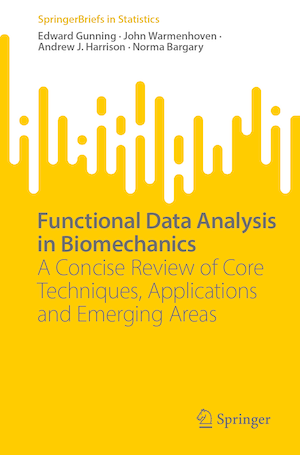
\includegraphics[width=0.175\linewidth]{figures/book_frontcover.png}
       \label{fig:enter-label}
   \end{figure}
\end{frame}

\begin{frame}[noframenumbering, allowframebreaks]{References}
       \printbibliography
\end{frame}

\end{document}